\documentclass{article}

\PassOptionsToPackage{numbers,sort&compress}{natbib}
\usepackage[preprint]{neurips}

\usepackage[utf8]{inputenc}
\usepackage[T1]{fontenc}
\usepackage{hyperref}
\usepackage{url}
\usepackage{booktabs}
\usepackage{amsfonts}
\usepackage{nicefrac}
\usepackage{microtype}
\usepackage{xcolor}
\usepackage{graphicx}
\usepackage{subcaption}
\usepackage{multirow}
\usepackage{array}
\usepackage{float}
\usepackage{adjustbox}
\usepackage{amsthm}
\usepackage{amsmath}
\usepackage{amssymb}
\usepackage{mathtools}
\usepackage{enumitem}
\usepackage{algorithm}
\usepackage{algpseudocode}
\usepackage{bbm}

\title{SWING: Source-Reweighting-Induced Eigen-Shrinkage for Single-Run Post-hoc Domain Generalization}
\author{Anonymous Authors}

\newtheorem{theorem}{Theorem}
\newtheorem{proposition}{Proposition}
\newtheorem{lemma}{Lemma}
\newtheorem{corollary}{Corollary}
\newtheorem{definition}{Definition}
\newtheorem{assumption}{Assumption}
\newtheorem{remark}{Remark}

\newcommand{\RR}{\mathbb{R}}
\newcommand{\EE}{\mathbb{E}}
\newcommand{\PP}{\mathbb{P}}
\newcommand{\cC}{\mathcal{C}}
\newcommand{\cQ}{\mathcal{Q}}
\newcommand{\cZ}{\mathcal{Z}}
\newcommand{\sZ}{\mathsf{Z}}
\newcommand{\argmin}{\operatorname*{arg\,min}}
\newcommand{\argmax}{\operatorname*{arg\,max}}
\newcommand{\diag}{\operatorname{diag}}
\newcommand{\rank}{\operatorname{rank}}
\newcommand{\tr}{\operatorname{tr}}
\newcommand{\barrier}{\operatorname{bar}}
\newcommand{\Cov}{\operatorname{Cov}}
\newcommand{\Var}{\operatorname{Var}}
\newcommand{\loss}{\ell}
\newcommand{\TBD}{\textbf{TBD}}
\newcommand{\swing}{\textup{\textsc{SWING}}}
\newcommand{\swad}{\textup{\textsc{SWAD}}}
\newcommand{\diwa}{\textup{\textsc{DiWA}}}
\newcommand{\miro}{\textup{\textsc{MIRO}}}
\newcommand{\erm}{\textup{\textsc{ERM}}}
\newcommand{\ood}{OOD}
\newcommand{\iid}{i.i.d.}
\newcommand{\norm}[1]{\left\lVert #1 \right\rVert}
\newcommand{\abs}[1]{\left\lvert #1 \right\rvert}
\newcommand{\paren}[1]{\left( #1 \right)}
\newcommand{\bracks}[1]{\left[ #1 \right]}
\newcommand{\braces}[1]{\left\{ #1 \right\}}
\newcommand{\inner}[2]{\left\langle #1, #2 \right\rangle}
\newcommand{\ip}[2]{\left\langle #1, #2 \right\rangle}
\newcommand{\one}{\mathbbm{1}}

\begin{document}

\maketitle

\begin{abstract}
Single-run post-hoc domain generalization is attractive because it can be attached to a strong empirical-risk-minimization pipeline without retraining. Existing post-hoc methods in this regime predominantly select or average checkpoints inside one connected low-loss region, motivated by flatness, locality, or diversity. This paper studies a different remaining degree of freedom: \emph{once a safe basin has already been found, should all directions inside that basin be trusted equally under domain shift?} We propose \textbf{\swing{}} (\textbf{S}ource-re\textbf{W}eighting-\textbf{I}nduced ei\textbf{N}-shrin\textbf{G}age), a single-run, post-hoc, domain-label-free method that learns a low-rank basin geometry from one dense checkpoint trajectory and then contracts only the directions that are fragile under plausible source-support reweightings. The method first constructs an anchor-centered barrier-filtered checkpoint pool, proves that this stage recovers a population-safe star basin up to explicit finite-sample margins, defines a basin center and trajectory subspace, fits a local quadratic source-risk surrogate on one held-out split, adds an explicit isotropic curvature inflation, estimates a reweighting fragility operator on a disjoint split, and finally outputs a single model by minimizing the resulting surrogate inside a basin trust region; when the constraint is inactive, this reduces to generalized eigen-shrinkage of the inflated baseline. We prove a local hidden-shift upper bound in which the reweighting term appears as a square-root variance penalty, show that any inflation level \(\tau\ge \sqrt{\varrho}K\) yields a valid quadratic hidden-shift certificate, derive exact minimax and dual representations of the robust surrogate, prove that smooth filtered basins are safe to average, quantify the exact gap to scalar shrinkage, establish stability for the constrained deployed estimator, and give finite-sample estimation rates for the source-fit and fragility operators together with a subspace truncation bound. The resulting theory is intentionally local: it certifies robustness to source-supported hidden reallocations inside the learned basin family rather than arbitrary support-expanding \ood{} shifts. The experimental sections intentionally leave all new \swing{} quantitative results as \TBD{}, while recording exact published benchmark context from prior work and providing the full evaluation protocol.
\end{abstract}

\section{Introduction}

Domain generalization (DG) asks for a predictor that performs well on an unseen target environment using only source data at training time. In practice, the DG methods that last are often the ones that preserve the base training recipe and change only how the final model is selected. This is why single-run post-hoc selection matters: one can train once, save dense checkpoints, and choose a deployable model after training has already finished.

Historically, \swad{} established checkpoint averaging as a serious DG tool by improving the average DomainBed ResNet-50 accuracy of \erm{} from \(63.3\) to \(66.9\) across PACS, VLCS, OfficeHome, TerraIncognita, and DomainNet \citep{cha2021swad}. Later work widened that picture. EoA studies moving-average model selection within a single run and heavier ensembles of averages across runs, reporting \(68.0\) average with a pre-trained ResNet-50 in its strongest setting \citep{arpit2022eoa}. More diverse weight-averaging schemes such as \diwa{} also reach \(68.0\) in heavier multi-run, multi-model configurations \citep{rame2022diwa}, a pretraining-aware method combined with the same post-hoc selector reaches \(68.1\) \citep{cha2022miro}, and the stronger non-post-hoc baseline \textsc{ERM++} reports \(68.9\) on the same ResNet-50 DomainBed suite \citep{teterwak2025ermpp}. WACV 2025 further reports stronger hybrid combinations on the same suite, including \diwa{}+\textsc{ERM++} at \(69.3\) and \miro{}+\textsc{ERM++} at \(69.4\) \citep{teterwak2025ermpp}. The empirical lesson is clear: the final predictor is often not the last checkpoint, and any new method now has to clear a stronger bar than the original \swad{} milestone.

Yet existing post-hoc DG methods still work inside one narrow action family. They select a checkpoint, an interval, or a soup inside a connected low-loss region. That is often enough to find a safe basin, but it leaves a natural question unanswered:
\begin{quote}
\textbf{After a safe basin has been identified, should the final model keep every direction inside that basin at full strength?}
\end{quote}

Our answer is no. Some directions inside a good basin are strongly supported by the pooled source data; others are fragile because small source-support redistributions would swing their contribution substantially. Those fragile directions are exactly the ones that should be attenuated before deployment.

This principle leads to \textbf{\swing{}} (\textbf{S}ource-re\textbf{W}eighting-\textbf{I}nduced ei\textbf{N}-shrin\textbf{G}age). \swing{} has two stages. First, it builds a safe connected checkpoint pool, computes a basin center, and extracts a low-rank trajectory subspace. Second, inside that subspace, it fits:
\begin{itemize}[leftmargin=1.4em]
    \item a \emph{source-fit operator} \(A_0\) that captures how strongly the pooled source data supports each direction,
    \item a \emph{fragility operator} \(B\) that measures how much examplewise local loss slopes vary across the source support, hence how strongly nearby source reweightings can swing the direction.
\end{itemize}
It then adds an explicit isotropic inflation \(A_\tau = A_0 + \tau I_r\) and minimizes the resulting surrogate inside the basin trust region. When the trust-region constraint is inactive, the edit reduces to shrinking the inflated baseline along the generalized eigenvectors of the pair \((B, A_\tau)\). The hidden-shift certificate corresponds to any \(\tau \ge \sqrt{\varrho}K\); in practice, \(\tau\) is an explicit inflation hyperparameter.

The central idea may be stated in one sentence:
\begin{quote}
\textbf{Directions that swing under plausible source reweightings should not survive deployment at full strength.}
\end{quote}

The scope of that claim is deliberately limited. The paper does not argue that source-only post-hoc editing can certify arbitrary \ood{} behavior. It argues that, \emph{within a safe basin and for target shifts that can be approximated as local redistributions of source support}, anisotropic suppression of reweighting-fragile directions is the natural next step after isotropic checkpoint averaging.

This move is still grounded in the current post-hoc DG literature. Weight averaging, mode connectivity, soups, and moving-average selectors tell us that dense trajectories often lie in a common low-loss basin \citep{izmailov2018swa,garipov2018fge,frankle2020linear,wortsman2022soups,arpit2022eoa}. Subspace-based Bayesian approximations further show that a small trajectory subspace can contain many high-performing models \citep{izmailov2020subspace}. Influence analyses and distributionally robust optimization show that sample reweightings are a natural first-order model of nearby distribution shifts \citep{koh2017influence,duchi2020variance,duchi2021learning}. \swing{} combines these threads into a post-hoc DG method that is still simple, still single-model at test time, and more directly tied to hidden shift than isotropic averaging.

We make six contributions.
\begin{enumerate}[leftmargin=1.4em]
    \item We introduce \swing{}, a single-run, post-hoc, domain-label-free DG method that performs a full-weight basin edit rather than another checkpoint selector.
    \item We prove that the anchor-based barrier filter used to construct the checkpoint pool recovers a population-safe star basin up to explicit concentration margins, and that any soup inside a smooth filtered basin obeys a concrete source-risk upper bound controlled by within-pool dispersion.
    \item We derive \swing{} from a local hidden-shift model in which target domains are source-supported \(\chi^2\)-bounded reweightings of the pooled source support. This yields a square-root fragility term \( \sqrt{\varrho\, z^\top B z}\), a certificate family of quadratic surrogates indexed by an isotropic inflation parameter \(\tau\ge \sqrt{\varrho}K\), and an exact minimax/dual interpretation of the resulting robust surrogate.
    \item We prove that the unconstrained inflated \swing{} edit has an exact generalized eigen-shrinkage form, and we quantify the exact gap between that anisotropic solution and the best scalar shrinkage rule inside the same quadratic model.
    \item We prove stability for the constrained deployed estimator that the algorithm actually returns, and we retain a sharper perturbation formula for the inactive-constraint special case.
    \item We give finite-sample estimation rates for the source-fit and fragility operators, a finite-sample bound for the deployed edit, and a subspace truncation theorem quantifying the price of restricting the method to the learned trajectory subspace.
\end{enumerate}

\begin{figure}[t]
    \centering
    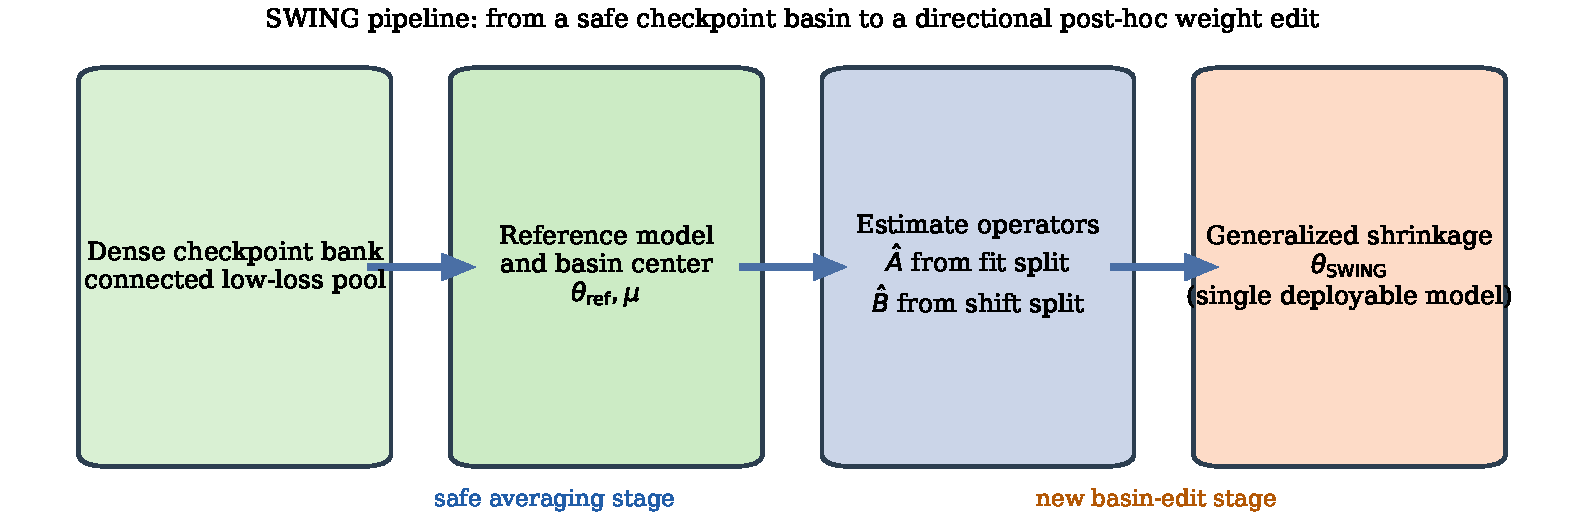
\includegraphics[width=\linewidth]{figures/method_overview.pdf}
    \caption{\textbf{\swing{} pipeline.} A dense checkpoint bank is reduced to a connected safe pool. That pool defines a basin center \(\mu\) and a low-rank subspace \(U\). On disjoint source splits, \swing{} estimates a source-fit operator \(\hat A_0\), inflates it to \(\hat A_\tau\), estimates a reweighting fragility operator \(\hat B\), and outputs one deployable model by minimizing the surrogate within the basin trust region; when the constraint is inactive, this reduces to generalized eigen-shrinkage of the inflated baseline.}
    \label{fig:overview}
\end{figure}

\section{Related Work}

\paragraph{Single-run post-hoc DG.}
\swad{} is the canonical checkpoint-averaging reference in single-run post-hoc DG \citep{cha2021swad}. EoA studies the same basic regime from a different angle: it uses moving averages within a run for model selection and also studies heavier ensembles of averages across runs, explicitly arguing that averaging can improve the correlation between validation and test performance \citep{arpit2022eoa}. Published follow-ups reinforce that post-hoc averaging is genuinely strong. At the same time, the strongest published \diwa{} configuration is explicitly heavier, averaging models from different training runs \citep{rame2022diwa}, while \miro{} improves the training representation and then benefits again from post-hoc selection \citep{cha2022miro}. \swing{} stays in the single-run deployment regime and changes the post-hoc action itself: it edits one final weight vector inside a safe basin rather than merely choosing which checkpoints to average.

\paragraph{Current benchmark landscape.}
The empirical bar has also moved. In addition to the historical \swad{}/\diwa{}/\miro{} milestones, \textsc{ERM++} shows that a carefully strengthened plain baseline reaches \(68.9\) average on the same ResNet-50 DomainBed suite, while hybrid combinations such as \diwa{}+\textsc{ERM++} and \miro{}+\textsc{ERM++} reach \(69.3\) and \(69.4\), respectively \citep{teterwak2025ermpp}. \swing{} is therefore not positioned against the 2021 landscape alone; it should be judged against both the post-hoc literature and stronger current baselines.

\paragraph{Weight averaging, connectivity, and basin geometry.}
Stochastic weight averaging \citep{izmailov2018swa}, fast geometric ensembling \citep{garipov2018fge}, linear mode connectivity \citep{frankle2020linear}, and model soups \citep{wortsman2022soups} show that dense training trajectories often traverse connected low-loss regions. Subspace inference further shows that a small trajectory subspace can contain many strong models \citep{izmailov2020subspace}. \swing{} uses these ideas as infrastructure: a connected checkpoint pool defines the basin, and a low-rank subspace provides the coordinate system for post-hoc editing.

\paragraph{Reweighting, influence, and local robustness.}
Influence functions quantify local sensitivity to sample reweightings \citep{koh2017influence}. Distributionally robust optimization studies worst-case risk over ambiguity sets such as \(\chi^2\) or other \(f\)-divergence balls \citep{duchi2016fdiv,duchi2020variance,duchi2021learning}. Closely related literatures study worst-case subpopulations, fairness without observed demographics, group-robust learning through reweighting, group-robust sample reweighting via influence functions, and unlabeled feature reweighting for group robustness \citep{li2021worstcase,hashimoto2018fairness,lahoti2020fairness,sagawa2020groupdro,qiao2025gsr,qiu2023afr}. Anchor regression is also relevant as a classical example of a structured shift-robust penalty rather than generic regularization \citep{rothenhausler2021anchor}. Tangent Prop is the classical precursor in input space: useful invariance can be enforced by controlling derivatives along nuisance directions \citep{simard1991tangent}. \swing{} transfers this logic to the empirical distribution: its nuisance directions are nearby redistributions of the source support.

\paragraph{Adjacent post-training weight editing outside DG.}
There is recent interest in editing weights after training to improve robustness or preserve \(\ood{}\) performance, including WiSE-FT interpolation, robustness signatures, model-stock averaging, and spectral soup editing \citep{wortsman2021wiseft,cai2023rws,jang2024modelstock,abdollahpoorrostam2026monosoup}. These works are adjacent but different. They do not target single-run post-hoc DG with source-only held-out data, do not derive a hidden-subpopulation reweighting geometry, and do not formulate the final edit as the solution of a basin-restricted hidden-shift surrogate whose unconstrained form is generalized eigen-shrinkage.

\section{Problem Setup}
\label{sec:setup}

We work in the standard source-only DG setting. Let \(P\) denote the pooled source distribution over examples \(Z=(X,Y)\). A dense training run produces checkpoints \(\theta_1,\dots,\theta_T \in \RR^d\). The method is post-hoc: training is already over, and only the checkpoints and held-out source data are used.

\paragraph{Safe checkpoint pool.}
Let \(S_{\mathrm{pool}}\) be a held-out source split used for pool construction. Define a source validation loss \(\widehat L_{\mathrm{pool}}(\theta)\) on this split. Let
\[
a \in \argmin_{1\le t \le T}\widehat L_{\mathrm{pool}}(\theta_t)
\]
be the empirical anchor checkpoint. For checkpoints \(i,j\), define the empirical interpolation barrier
\[
\barrier(i,j)
=
\max_{\alpha\in\mathcal G}
\widehat L_{\mathrm{pool}}\paren{\alpha \theta_i + (1-\alpha)\theta_j}
-
\max\braces{\widehat L_{\mathrm{pool}}(\theta_i),\widehat L_{\mathrm{pool}}(\theta_j)},
\]
where \(\mathcal G \subset [0,1]\) is a fixed interpolation grid. For user-chosen thresholds \(\varepsilon_{\mathrm{pool}}, \tau_{\mathrm{pool}} > 0\), define the safe pool
\[
\cC
=
\braces{
t : \widehat L_{\mathrm{pool}}(\theta_t) \le \widehat L_{\mathrm{pool}}(\theta_a) + \varepsilon_{\mathrm{pool}},
\ \barrier(t,a)\le \tau_{\mathrm{pool}}
}.
\]
This pool is intended to isolate one connected low-loss basin through an anchor-centered barrier filter. We write
\[
\mathfrak{S}_a(\cC)
=
\bigcup_{t\in\cC}
\braces{(1-\alpha)\theta_a + \alpha \theta_t : \alpha\in[0,1]}
\]
for the star hull traced out by anchor-to-candidate interpolation paths, and
\[
\operatorname{conv}(\cC)
=
\braces{
\sum_{t\in\cC} w_t \theta_t :
w_t\ge 0,\ \sum_{t\in\cC} w_t = 1
}
\]
for the soup hull of the retained pool. The pool construction stage is not the novelty of the paper; it is the infrastructure on top of which \swing{} operates.

\paragraph{Basin coordinates.}
Define the basin center
\[
\mu = \frac{1}{|\cC|}\sum_{t\in\cC}\theta_t.
\]
Let \(U\in\RR^{d\times r}\) have orthonormal columns spanning the top \(r\) principal components of \(\braces{\theta_t-\mu : t\in\cC}\). Every point \(z\in\RR^r\) induces a full model
\[
\theta(z)=\mu + Uz.
\]
The safe pool itself induces observed coordinates
\[
z_t = U^\top(\theta_t - \mu), \qquad t\in\cC.
\]
For every such coordinate, we also define the projected subspace model
\[
\tilde\theta_t = \theta(z_t) = \mu + U z_t, \qquad t\in\cC.
\]

\paragraph{Disjoint source splits.}
Beyond \(S_{\mathrm{pool}}\), \swing{} uses two disjoint held-out source splits:
\begin{itemize}[leftmargin=1.4em]
    \item \(S_{\mathrm{fit}}\), used to fit a local quadratic source-risk surrogate;
    \item \(S_{\mathrm{shift}}\), used to estimate the fragility operator.
\end{itemize}
The split separation is deliberate: it reduces direct reuse of the same source examples when fitting the source geometry and the hidden-shift geometry, although it does not by itself guarantee independence or unbiasedness once the upstream checkpoint pool and subspace have already been selected.

In theory, \(\cZ\) is any compact convex trust region containing the observed safe-pool coordinates. In practice, we instantiate \(\cZ\) as a box in subspace coordinates whose sides are determined by the extrema of the safe-pool projections.

\section{The Method}
\label{sec:method}

\subsection{Quadratic source-fit surrogate}

Choose a local fitting neighborhood
\[
\cC_{\mathrm{loc}}
=
\braces{t\in\cC : \norm{z_t}\le \rho_{\mathrm{loc}}}
\]
for a user-chosen radius \(\rho_{\mathrm{loc}}>0\). On \(S_{\mathrm{fit}}\), \swing{} fits a local quadratic model of source risk in the basin subspace:
\[
q_0(z) = c + a^\top z + \frac{1}{2} z^\top A_0 z,
\qquad
A_0 \in \RR^{r\times r}, \ A_0 \succ 0.
\]
In practice, \(q_0\) is estimated from the local projected-model cloud \(\braces{(z_t,\tilde\theta_t) : t\in\cC_{\mathrm{loc}}}\) by least-squares fitting of the empirical losses
\[
\widehat L_{\mathrm{fit}}(\tilde\theta_t)
\approx
c + a^\top z_t + \frac{1}{2} z_t^\top A_0 z_t.
\]
The unique minimizer of the quadratic fit-only surrogate is
\[
z_{\mathrm{fit}} = -A_0^{-1}a.
\]
This is the source-fit solution in the basin coordinate system.

\subsection{Fragility operator from source reweightings}

Fix an example \(Z_i \in S_{\mathrm{shift}}\). Let \(\phi_i \in \RR^r\) denote the local first-order loss slope of that example in the basin subspace. Formally, in the theory we assume
\[
\loss\paren{\theta(z); Z_i}
=
\loss\paren{\theta(0); Z_i}
+
\phi_i^\top z
+
r_i(z),
\]
with a controlled quadratic remainder \(r_i(z)\).

The fragility operator is the covariance of these examplewise slopes:
\[
B
=
\Cov(\phi)
=
\EE\bracks{(\phi - \EE[\phi])(\phi-\EE[\phi])^\top}.
\]
Intuitively:
\begin{itemize}[leftmargin=1.4em]
    \item if a direction has small variance in examplewise slopes, then nearby source reweightings do not change its preferred update much;
    \item if a direction has large variance, then small hidden redistributions of the source support can swing its utility sharply.
\end{itemize}

In practice, \(\phi_i\) is estimated locally around \(z=0\), not from the entire checkpoint cloud. For each example \(Z_i\), \swing{} fits a local quadratic model on \(\cC_{\mathrm{loc}}\),
\[
\loss(\tilde\theta_t;Z_i)
\approx
\alpha_i + \hat\phi_i^\top z_t + \frac12 z_t^\top \hat H_i z_t,
\qquad t\in\cC_{\mathrm{loc}},
\]
and takes the fitted linear coefficient \(\hat\phi_i\) as the estimated derivative at the basin center. The empirical fragility operator \(\hat B\) is then the sample covariance of these local slope estimates.

\subsection{The \swing{} objective}

For any inflation level \(\tau\ge 0\), define
\[
A_\tau = A_0 + \tau I_r.
\]
The derivation in Section~\ref{sec:theory} yields a \emph{family} of quadratic hidden-shift surrogates
\[
J_{\lambda,\tau}(z)
=
a^\top z + \frac12 z^\top A_\tau z + \frac{\lambda}{2} z^\top B z,
\qquad \lambda > 0,\ \tau\ge 0.
\]
The first two terms combine source fit with isotropic curvature inflation. The third term penalizes directions whose first-order contribution is unstable under plausible source-support reweightings. In the hidden-shift theory, every \(\tau\ge \sqrt{\varrho}K\) is certificate-compatible; in practice \(\tau\) is an explicit hyperparameter.

The analyzed population surrogate minimizer is
\[
z_{\lambda,\tau}^{\cZ}
\in
\argmin_{z\in\cZ} J_{\lambda,\tau}(z).
\]
Whenever the unconstrained minimizer lies inside \(\cZ\), the constrained and unconstrained solutions coincide.

Given empirical plug-in estimates \((\hat a,\hat A_0,\hat B)\), define
\[
\hat A_\tau = \hat A_0 + \tau I_r,
\qquad
\hat J_{\lambda,\tau}(z)
=
\hat a^\top z + \frac12 z^\top \hat A_\tau z + \frac{\lambda}{2} z^\top \hat B z.
\]
The practical returned estimator is the constrained empirical plug-in minimizer
\[
\hat z_{\lambda,\tau}^{\cZ}
\in
\argmin_{z\in\cZ} \hat J_{\lambda,\tau}(z).
\]

Let
\[
z_\tau=-A_\tau^{-1}a.
\]
Then
\[
J_{\lambda,\tau}(z)
=
\text{const}
+
\frac12 (z-z_\tau)^\top A_\tau (z-z_\tau)
+
\frac{\lambda}{2} z^\top B z.
\]
Therefore \swing{} should be interpreted as a \emph{basin edit}: it does not search for a new basin, but contracts an inflated local baseline along fragile directions inside a basin that was already judged safe by the first-stage pool construction.

\subsection{Generalized eigen-shrinkage}

Because \(A_\tau\succ 0\) and \(B\succeq 0\), there exists an \(A_\tau\)-orthonormal generalized eigenbasis \(V=[v_1,\dots,v_r]\) and nonnegative generalized eigenvalues \(\nu_1,\dots,\nu_r\) such that
\[
Bv_j = \nu_j A_\tau v_j,
\qquad
V^\top A_\tau V = I.
\]
Writing
\[
z_\tau = \sum_{j=1}^r c_j v_j,
\qquad
c_j = v_j^\top A_\tau z_\tau,
\]
the unconstrained \swing{} edit is
\[
z_{\lambda,\tau}^{\mathrm{unc}} = \sum_{j=1}^r \frac{c_j}{1+\lambda \nu_j}v_j.
\]
Thus every generalized coordinate is shrunk by a factor
\[
\beta_j(\lambda)=\frac{1}{1+\lambda\nu_j}.
\]
Directions with larger fragility-to-fit ratio \(\nu_j\) receive stronger attenuation.

\begin{algorithm}[t]
\caption{\swing{}}
\label{alg:swing}
\begin{algorithmic}[1]
\Require Dense checkpoint bank \(\braces{\theta_t}_{t=1}^T\), held-out source splits \(S_{\mathrm{pool}},S_{\mathrm{fit}},S_{\mathrm{shift}}\), rank \(r\), thresholds \(\varepsilon_{\mathrm{pool}},\tau_{\mathrm{pool}}\), local radius \(\rho_{\mathrm{loc}}\), regularization \(\lambda\), inflation \(\tau\).
\State Select the safe checkpoint pool \(\cC\) using source-fit thresholding and interpolation barriers on \(S_{\mathrm{pool}}\).
\State Compute the basin center \(\mu = |\cC|^{-1}\sum_{t\in\cC}\theta_t\).
\State Compute \(U\in\RR^{d\times r}\) from the top \(r\) principal directions of \(\braces{\theta_t-\mu : t\in\cC}\).
\State Form checkpoint coordinates \(z_t = U^\top(\theta_t-\mu)\), \(t\in\cC\).
\State Define projected subspace models \(\tilde\theta_t = \mu + U z_t\), \(t\in\cC\).
\State Keep the local neighborhood \(\cC_{\mathrm{loc}}=\braces{t\in\cC : \norm{z_t}\le \rho_{\mathrm{loc}}}\).
\State Fit the local quadratic source-risk surrogate \(q_0(z)=c+a^\top z+\tfrac12 z^\top A_0 z\) on \(S_{\mathrm{fit}}\) using the projected models \(\tilde\theta_t\), \(t\in\cC_{\mathrm{loc}}\).
\State Form the inflated fit operator \(\hat A_\tau = \hat A_0 + \tau I_r\).
\State Fit local examplewise quadratic models on \(S_{\mathrm{shift}}\) over the projected models \(\tilde\theta_t\), \(t\in\cC_{\mathrm{loc}}\), extract linear coefficients \(\hat\phi_i\), and set \(\hat B = \widehat{\Cov}(\hat\phi)\).
\State Define the empirical plug-in objective \(\hat J_{\lambda,\tau}(z)=\hat a^\top z+\tfrac12 z^\top \hat A_\tau z+\tfrac{\lambda}{2} z^\top \hat B z\).
\State Solve the generalized eigenproblem \(\hat B v_j = \nu_j \hat A_\tau v_j\), \(V^\top \hat A_\tau V = I\).
\State Compute \(\hat z_\tau = -\hat A_\tau^{-1}\hat a\) and coefficients \(\hat c_j = v_j^\top \hat A_\tau \hat z_\tau\).
\State Set the unconstrained empirical edit \(\hat z_{\lambda,\tau}^{\mathrm{unc}} = \sum_{j=1}^r \frac{\hat c_j}{1+\lambda \nu_j}v_j\).
\State If \(\hat z_{\lambda,\tau}^{\mathrm{unc}}\in\cZ\), set \(\hat z_{\lambda,\tau}^{\cZ}=\hat z_{\lambda,\tau}^{\mathrm{unc}}\); otherwise solve \(\hat z_{\lambda,\tau}^{\cZ}\in\argmin_{z\in\cZ} \hat J_{\lambda,\tau}(z)\) inside the chosen trust region.
\State \Return \(\theta_{\mathrm{SWING}} = \mu + U \hat z_{\lambda,\tau}^{\cZ}\).
\end{algorithmic}
\end{algorithm}

\begin{figure*}[t]
    \centering
    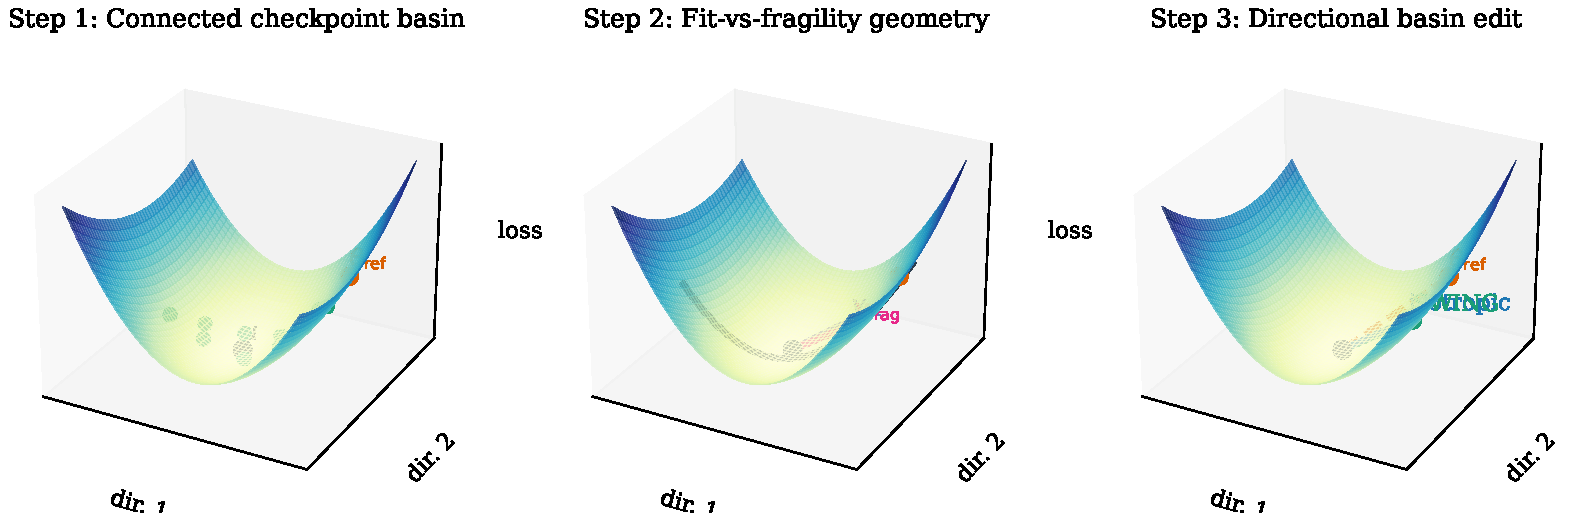
\includegraphics[width=0.92\textwidth]{figures/basin_3d_steps.pdf}
    \caption{\textbf{Three-dimensional intuition for \swing{}.} Left: dense checkpoints define a connected low-loss basin and a center \(\mu\). Middle: the basin subspace supplies the coordinates in which the local fit, isotropic inflation, and fragility are estimated. Right: \swing{} contracts the inflated baseline anisotropically, suppressing high-fragility directions more than low-fragility directions.}
    \label{fig:basin3d}
\end{figure*}

\section{Theory}
\label{sec:theory}

This section now has two jobs. First, it formalizes why anchor-based barrier filtering identifies a star basin whose retained checkpoints are low-risk and low-barrier, and why averaging inside that basin is safe once the additional convex-hull smoothness condition is imposed. Second, it derives the \swing{} edit from a local hidden-shift model and strengthens the estimator theory beyond the original unconstrained plug-in argument.

\subsection{Barrier-filtered basins and soup safety}

The safe-pool stage is not the novelty of \swing{}, but it is the mathematical infrastructure the directional edit relies on. The next results make precise what such a barrier filter certifies.

\begin{theorem}[Barrier-filtered pool is population-safe on the interpolation grid]
\label{thm:pool_filter}
Assume that \(S_{\mathrm{pool}}\) consists of i.i.d.\ examples from \(P\) and that every loss evaluated at a checkpoint \(\theta_t\) or at a grid interpolation point \((1-\alpha)\theta_i + \alpha \theta_j\) with \(i,j\in[T]\) and \(\alpha\in\mathcal G\) lies in \([0,L_{\max}^{\mathrm{pool}}]\). Let \(a\) and \(\cC\) be the empirical anchor and empirical safe pool from Section~\ref{sec:setup}, and define
\[
\xi_{\mathrm{pool}}(\delta)
=
L_{\max}^{\mathrm{pool}}
\sqrt{
\frac{\log\!\paren{2\paren{T+T^2\abs{\mathcal G}}/\delta}}{2\abs{S_{\mathrm{pool}}}}
}.
\]
Then, with probability at least \(1-\delta\),
\[
L_P(\theta_a)
\le
\min_{1\le t\le T} L_P(\theta_t) + 2\xi_{\mathrm{pool}}(\delta),
\]
and every \(t\in\cC\) satisfies
\[
L_P(\theta_t)
\le
L_P(\theta_a) + \varepsilon_{\mathrm{pool}} + 2\xi_{\mathrm{pool}}(\delta),
\]
\[
\max_{\alpha\in\mathcal G}
L_P\paren{(1-\alpha)\theta_a + \alpha \theta_t}
\le
\max\braces{L_P(\theta_a),L_P(\theta_t)}
+
\tau_{\mathrm{pool}} + 2\xi_{\mathrm{pool}}(\delta).
\]
\end{theorem}

Theorem~\ref{thm:pool_filter} already gives a rigorous finite-sample statement for the random pool-building stage: the empirical barrier filter recovers a star pool whose checkpoints are population-near-optimal and population-low-barrier up to explicit concentration margins.

\begin{corollary}[Full-segment safety from a finite interpolation grid]
\label{cor:segment_barrier}
Let
\[
\gamma(\mathcal G)
=
\sup_{u\in[0,1]} \min_{\alpha\in\mathcal G} \abs{u-\alpha}
\]
be the mesh width of the interpolation grid. Under the event of Theorem~\ref{thm:pool_filter}, assume additionally that \(L_P\) is differentiable on the star hull \(\mathfrak{S}_a(\cC)\) and that
\[
\sup_{\theta\in \mathfrak{S}_a(\cC)} \norm{\nabla L_P(\theta)} \le G_{\mathrm{pool}}.
\]
Then every \(t\in\cC\) satisfies
\[
\sup_{\alpha\in[0,1]}
L_P\paren{(1-\alpha)\theta_a + \alpha \theta_t}
\le
\max\braces{L_P(\theta_a),L_P(\theta_t)}
+
\tau_{\mathrm{pool}} + 2\xi_{\mathrm{pool}}(\delta)
+
G_{\mathrm{pool}} \norm{\theta_t-\theta_a}\,\gamma(\mathcal G).
\]
\end{corollary}

Corollary~\ref{cor:segment_barrier} closes the grid-discretization gap: a finite interpolation grid certifies the full anchor-to-candidate segment whenever source risk does not change too sharply between adjacent grid points.

\begin{theorem}[Safe averaging inside a smooth filtered basin]
\label{thm:soup_safe}
Assume \(L_P\) is twice continuously differentiable on the soup hull \(\operatorname{conv}(\cC)\) and that
\[
\nabla^2 L_P(\theta) \succeq -\beta_{\mathrm{pool}} I_d
\qquad
\text{for all } \theta\in\operatorname{conv}(\cC).
\]
For any weights \((w_t)_{t\in\cC}\) satisfying \(w_t\ge 0\) and \(\sum_{t\in\cC} w_t=1\), define
\[
\theta_w = \sum_{t\in\cC} w_t \theta_t.
\]
Then
\[
L_P(\theta_w)
\le
\sum_{t\in\cC} w_t L_P(\theta_t)
+
\frac{\beta_{\mathrm{pool}}}{2}
\sum_{t\in\cC} w_t \norm{\theta_t-\theta_w}^2.
\]
In particular, if every \(t\in\cC\) obeys
\[
L_P(\theta_t) \le L_P(\theta_a) + \varepsilon_{\mathrm{safe}},
\]
then
\[
L_P(\theta_w)
\le
L_P(\theta_a)
+
\varepsilon_{\mathrm{safe}}
+
\frac{\beta_{\mathrm{pool}}}{2}
\sum_{t\in\cC} w_t \norm{\theta_t-\theta_w}^2.
\]
\end{theorem}

Theorem~\ref{thm:soup_safe} is the precise sense in which barrier-screened post-hoc methods identify checkpoints that are safe to average: once the retained cloud stays in a smooth common basin, the source loss of any soup is controlled by the retained endpoint losses plus an explicit within-pool variance term.

\subsection{Hidden-shift assumptions}

\begin{assumption}[Local quadratic source-fit model]
\label{ass:fit}
There exists a compact convex set \(\cZ \subset \RR^r\) containing \(0\) and the observed checkpoint coordinates, and a positive definite matrix \(A_0\in\RR^{r\times r}\) and vector \(a\in\RR^r\) such that the pooled source excess risk on the basin subspace satisfies
\[
L_P(z) - L_P(0)
=
a^\top z + \frac12 z^\top A_0 z
\qquad
\text{for all } z\in\cZ.
\]
Moreover \(L_P(z)\) and \(L_Q(z)\) are finite for all \(z\in\cZ\) and all \(Q\in\cQ(\varrho)\).
\end{assumption}

\begin{assumption}[Examplewise local linearization with quadratic remainder]
\label{ass:lin}
There exist measurable \(\phi : \sZ\to\RR^r\) and \(\kappa : \sZ\to[0,\infty)\) such that for every example \(Z\in\sZ\) and every \(z\in\cZ\),
\[
\loss(\theta(z);Z)
=
\loss(\theta(0);Z)
+
\phi(Z)^\top z
+
r(Z,z),
\]
where the remainder satisfies
\[
\abs{r(Z,z)} \le \frac{\kappa(Z)}{2}\norm{z}^2
\qquad
\text{for all } z\in\cZ.
\]
Moreover \(\EE_P[\norm{\phi(Z)}^2] < \infty\) and
\(\EE_P[\kappa(Z)^2] \le K^2 < \infty\).
\end{assumption}

\begin{assumption}[Source-supported local target shift]
\label{ass:shift}
The target distribution \(Q\) is absolutely continuous with respect to \(P\) and belongs to the local \(\chi^2\)-style ambiguity family
\[
\cQ(\varrho)
=
\braces{
Q : \frac{dQ}{dP} = 1+h,\ 1+h\ge 0 \text{ $P$-a.s.},\ \EE_P[h]=0,\ \EE_P[h^2]\le \varrho
}
\]
for some radius \(\varrho \ge 0\).
\end{assumption}

Assumption~\ref{ass:shift} encodes the source-supported hidden-subpopulation view: unseen domains are local redistributions of source support mass. It is therefore a deliberately local model of DG, not a claim that every realistic target environment is source-supported. Assumption~\ref{ass:lin} makes that redistribution observable through the examplewise slope covariance. Assumption~\ref{ass:fit} isolates the source-fit geometry inside the safe basin found in the first stage.

\subsection{Deriving the fragility term}

\begin{theorem}[Local hidden-shift upper bound]
\label{thm:robust_bound}
Under Assumptions~\ref{ass:fit}--\ref{ass:shift}, define
\[
\bar\phi = \EE_P[\phi(Z)],
\qquad
B = \Cov_P(\phi(Z))
=
\EE_P\bracks{(\phi(Z)-\bar\phi)(\phi(Z)-\bar\phi)^\top}.
\]
Then for every \(z\in\cZ\) and every \(Q\in\cQ(\varrho)\),
\[
L_Q(z)
\le
L_Q(0)
+
a^\top z + \frac12 z^\top A_0 z
+
\sqrt{\varrho\, z^\top B z}
+
\frac{\sqrt{\varrho}\,K}{2}\norm{z}^2.
\]
\end{theorem}

Theorem~\ref{thm:robust_bound} shows exactly where the fragility term comes from. The quantity \(z^\top B z\) is the variance of the first-order examplewise slope in direction \(z\). If that variance is large, local source reweightings can swing the contribution of \(z\) strongly; if it is small, the direction is reweighting-stable.

\begin{corollary}[Quadratic \swing{} surrogate]
\label{cor:quadratic_majorizer}
Under the assumptions of Theorem~\ref{thm:robust_bound}, for every \(\lambda>0\) and every \(\tau\ge \sqrt{\varrho}K\),
\[
L_Q(z)
\le
L_Q(0) + \frac{\varrho}{2\lambda}
+
a^\top z
+
\frac12 z^\top A_\tau z
+
\frac{\lambda}{2} z^\top B z
\qquad
\text{for all } z\in\cZ,
\]
where
\[
A_\tau = A_0 + \tau I_r.
\]
\end{corollary}

Corollary~\ref{cor:quadratic_majorizer} is the exact bridge from the hidden-shift model to \swing{}: for each fixed \(\lambda>0\), Young's inequality yields a quadratic upper bound, and \(\lambda\) controls the tradeoff between the additive constant and the fragility penalty. The hidden-shift certificate remains valid for any isotropic inflation \(\tau\ge \sqrt{\varrho}K\). Equivalently, for any chosen inflation level \(\tau\), the same bound certifies all local source-supported shifts whose ambiguity radius satisfies \(\varrho \le (\tau/K)^2\). In practice, \(\tau\) is therefore best read as a conservativeness knob that indexes a family of certified local shift radii rather than as an oracle quantity inferred from the target domain.

\begin{proposition}[Exact minimax and dual representations]
\label{prop:minimax}
Define the local robust surrogate
\[
R_{\varrho,\tau}(z)
=
a^\top z + \frac12 z^\top A_\tau z + \sqrt{\varrho\, z^\top B z}.
\]
Then, for every \(z\in\cZ\),
\[
R_{\varrho,\tau}(z)
=
\sup_{\norm{u}_2\le \sqrt{\varrho}}
\bracks{
a^\top z + \frac12 z^\top A_\tau z + u^\top B^{1/2} z
}
=
\inf_{\lambda>0}
\bracks{
\frac{\varrho}{2\lambda} + J_{\lambda,\tau}(z)
}.
\]
\end{proposition}

Proposition~\ref{prop:minimax} strengthens the interpretation of \swing{}. The square-root surrogate is the exact value of a local adversarial linear game in the fragility coordinates, while the quadratic objective \(J_{\lambda,\tau}\) is its exact one-parameter dual relaxation.

\subsection{Closed-form shrinkage solution}

\begin{theorem}[Generalized eigen-shrinkage]
\label{thm:closed_form}
Let
\[
J_{\lambda,\tau}(z)=a^\top z + \frac12 z^\top A_\tau z + \frac{\lambda}{2} z^\top B z,
\qquad
A_\tau = A_0 + \tau I_r,\ A_\tau\succ 0,\ B\succeq 0,\ \lambda>0,\ \tau\ge 0.
\]
Define the inflated baseline
\[
z_\tau = -A_\tau^{-1}a.
\]
Then:
\begin{enumerate}[leftmargin=1.4em]
    \item The unconstrained problem \(\min_{z\in\RR^r} J_{\lambda,\tau}(z)\) is strongly convex and has the unique minimizer
    \[
    z_{\lambda,\tau}^{\mathrm{unc}} = -(A_\tau+\lambda B)^{-1}a = (A_\tau+\lambda B)^{-1}A_\tau z_\tau.
    \]
    \item If \(z_{\lambda,\tau}^{\mathrm{unc}}\in\cZ\), then \(z_{\lambda,\tau}^{\cZ}=z_{\lambda,\tau}^{\mathrm{unc}}\). In that case, if \(V=[v_1,\dots,v_r]\) is an \(A_\tau\)-orthonormal generalized eigenbasis satisfying
    \[
    Bv_j = \nu_j A_\tau v_j,
    \qquad
    V^\top A_\tau V = I,
    \qquad
    \nu_j\ge 0,
    \]
    and
    \[
    z_\tau = \sum_{j=1}^r c_j v_j,
    \qquad
    c_j = v_j^\top A_\tau z_\tau,
    \]
    then
    \[
    z_{\lambda,\tau}^{\cZ} = z_{\lambda,\tau}^{\mathrm{unc}} = \sum_{j=1}^r \frac{c_j}{1+\lambda\nu_j}v_j.
    \]
\end{enumerate}
\end{theorem}

Theorem~\ref{thm:closed_form} is the central algebraic result of the paper. It shows that \swing{} is not merely a heuristic penalty. Whenever the unconstrained minimizer stays inside the chosen basin trust region, the analyzed population solution is an exact contraction of the inflated baseline, with one shrinkage factor per generalized fragility level.

\begin{figure}[t]
    \centering
    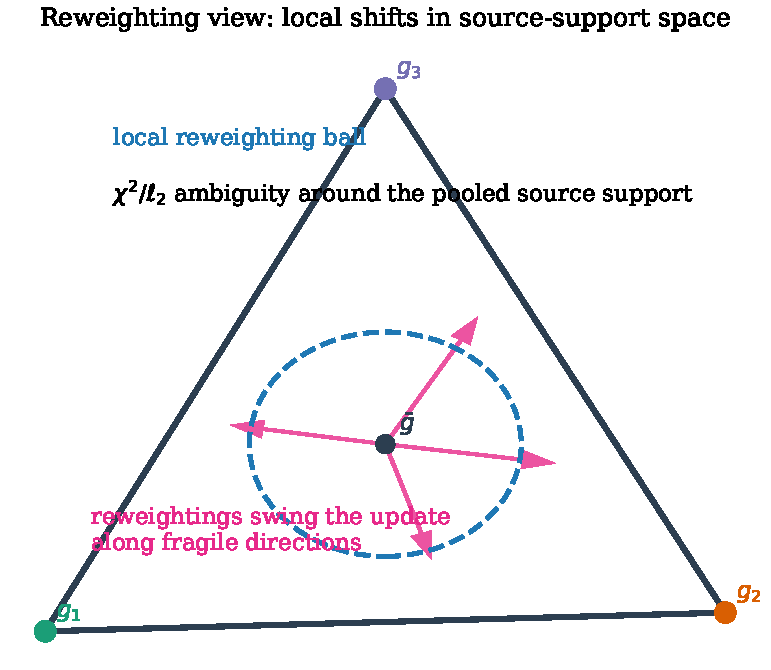
\includegraphics[width=0.92\linewidth]{figures/reweighting_simplex.pdf}
    \caption{\textbf{Why reweighting induces a fragility operator.} Nearby target domains are modeled as local redistributions of source-support mass. Examplewise slope vectors that fan out strongly under these redistributions produce a large covariance \(B\), so directions aligned with them are shrunk more aggressively by \swing{}.}
    \label{fig:simplex}
\end{figure}

\subsection{Why anisotropy matters}

The next comparison result quantifies the price of using only one global shrinkage factor when fragility is heterogeneous across the basin subspace.

\begin{proposition}[Quantitative gap to scalar shrinkage]
\label{prop:scalar_gap}
Under the assumptions of Theorem~\ref{thm:closed_form}, consider the scalar shrinkage family
\[
\mathcal F_{\mathrm{sc}}
=
\braces{\alpha z_\tau : \alpha\in\RR}.
\]
If \(z_\tau = 0\), then \(\min_{\alpha} J_{\lambda,\tau}(\alpha z_\tau)=J_{\lambda,\tau}(z_{\lambda,\tau}^{\mathrm{unc}})\). Otherwise define
\[
S = \sum_{j=1}^r c_j^2,
\qquad
p_j = \frac{c_j^2}{S},
\qquad
f_\lambda(\nu)=\frac{1}{1+\lambda \nu}.
\]
Then
\[
\Delta_{\mathrm{sc}}
:=
\min_{\alpha\in\RR} J_{\lambda,\tau}(\alpha z_\tau)
-
J_{\lambda,\tau}(z_{\lambda,\tau}^{\mathrm{unc}})
=
\frac{S}{2}
\bracks{
\sum_{j=1}^r p_j f_\lambda(\nu_j)
-
f_\lambda\!\paren{\sum_{j=1}^r p_j \nu_j}
}.
\]
Consequently \(\Delta_{\mathrm{sc}}\ge 0\), with equality if and only if the generalized eigenvalues \(\nu_j\) are constant on the support of \(z_\tau\). If
\[
\nu_{\max}^{\mathrm{act}} = \max\braces{\nu_j : c_j\neq 0},
\]
then
\[
\Delta_{\mathrm{sc}}
\ge
\frac{S\lambda^2}{2\paren{1+\lambda \nu_{\max}^{\mathrm{act}}}^3}
\Var_p(\nu),
\qquad
\Var_p(\nu)=\sum_{j=1}^r p_j\paren{\nu_j-\sum_{k=1}^r p_k\nu_k}^2.
\]
\end{proposition}

Proposition~\ref{prop:scalar_gap} shows more than a yes-or-no comparison. The advantage of anisotropic shrinkage grows quantitatively with the weighted dispersion of the active fragility-to-fit ratios.

\begin{figure}[t]
    \centering
    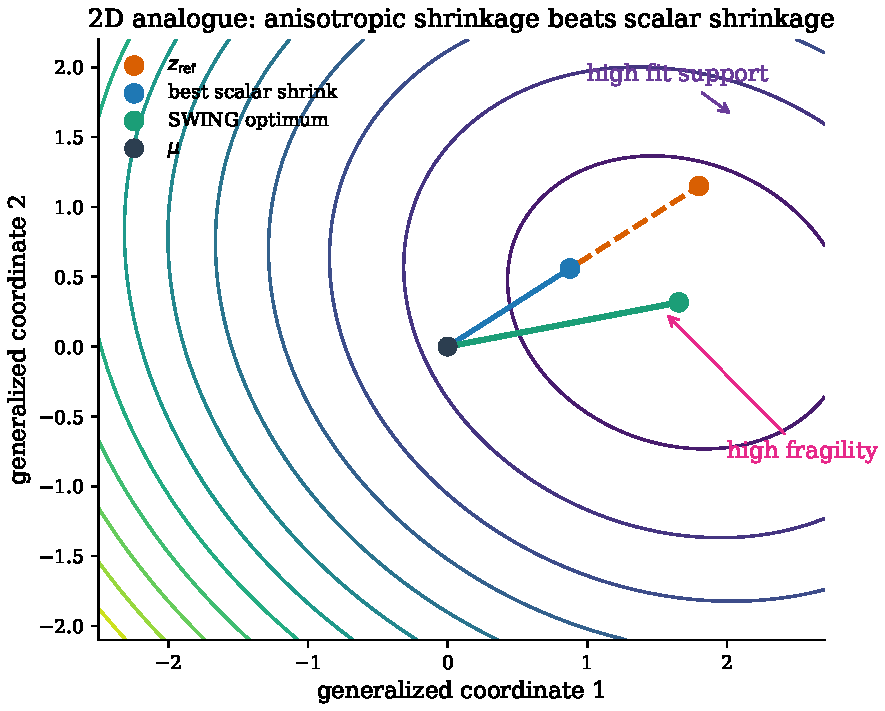
\includegraphics[width=0.95\linewidth]{figures/anisotropic_vs_scalar_2d.pdf}
    \caption{\textbf{Two-dimensional analogue of Proposition~\ref{prop:scalar_gap}.} The inflated baseline \(z_\tau\) lies away from the basin center \(\mu\). The best scalar shrinkage moves only along the dashed ray. The \swing{} optimum follows the anisotropic geometry defined by \(A_\tau\) and \(B\), producing a lower robust surrogate value whenever fragility is direction-dependent.}
    \label{fig:2d}
\end{figure}

\subsection{Certificate improvement, estimation, and stability}

\begin{proposition}[Exact certificate gain over the inflated baseline]
\label{prop:gain}
Under the assumptions of Theorem~\ref{thm:closed_form},
\[
J_{\lambda,\tau}(z_\tau) - J_{\lambda,\tau}(z_{\lambda,\tau}^{\mathrm{unc}})
=
\frac12 (z_\tau-z_{\lambda,\tau}^{\mathrm{unc}})^\top (A_\tau+\lambda B)(z_\tau-z_{\lambda,\tau}^{\mathrm{unc}}).
\]
In particular,
\[
J_{\lambda,\tau}(z_{\lambda,\tau}^{\mathrm{unc}})\le J_{\lambda,\tau}(z_\tau),
\]
with equality if and only if \(B z_\tau = 0\).
\end{proposition}

Proposition~\ref{prop:gain} quantifies the exact improvement that \swing{} certifies over the inflated baseline. If that baseline already lies in the kernel of the fragility operator, there is nothing to shrink; otherwise the robust surrogate is improved strictly.

\begin{theorem}[Constrained argmin stability]
\label{thm:constrained}
Let
\[
M = A_\tau+\lambda B,
\qquad
\hat M = \hat A_\tau + \lambda \hat B,
\qquad
m = \lambda_{\min}(M),
\qquad
D_\cZ = \sup_{z\in\cZ}\norm{z}.
\]
Suppose \(m>0\), \(\hat M\succeq 0\), and define
\[
\delta = \norm{\hat A_\tau - A_\tau} + \lambda \norm{\hat B-B}.
\]
Let
\[
z_{\lambda,\tau}^{\cZ}
\in
\argmin_{z\in\cZ}
\bracks{a^\top z + \frac12 z^\top M z},
\qquad
\hat z_{\lambda,\tau}^{\cZ}
\in
\argmin_{z\in\cZ}
\bracks{\hat a^\top z + \frac12 z^\top \hat M z}.
\]
Then
\[
\norm{\hat z_{\lambda,\tau}^{\cZ} - z_{\lambda,\tau}^{\cZ}}
\le
\frac{\norm{\hat a-a} + D_\cZ \delta}{m}.
\]
\end{theorem}

Theorem~\ref{thm:constrained} is the deployed-estimator stability result: it covers the constrained model actually returned by the algorithm, not only the inactive-trust-region case.

\begin{assumption}[Conditional local identification for plug-in estimation]
\label{ass:identify}
For the estimation discussion only, condition on a deterministic asymptotic sequence of upstream-selected basin families \((\mu_n,U_n,\cC_n,\cC_{\mathrm{loc},n},\cZ_n)\). Assume that \(0\) lies in the interior of the convex hull of every local coordinate design, that the local polynomial Gram matrices formed by the intercept, linear monomials, and quadratic monomials over \(\cC_{\mathrm{loc},n}\) are uniformly well conditioned, and that the fill distance of the local design around \(0\) tends to zero along the sequence. Assume further that the examplewise losses restricted to each basin family are three times continuously differentiable with uniformly bounded third derivatives on a neighborhood of \(0\).
\end{assumption}

Assumption~\ref{ass:identify} is not used in the algebraic population certificate. It is only the local-regularity condition needed to interpret the practical ridge regressions as derivative estimators inside a fixed basin family.

\begin{theorem}[Source-fit operator estimation]
\label{thm:A_est}
Let
\[
p = 1 + r + \frac{r(r+1)}{2},
\]
and let \(\psi:\RR^r\to\RR^p\) collect the intercept, linear monomials, and unique quadratic monomials with the convention that for every scalar \(c\), vector \(a\), and symmetric matrix \(A\), if \(\beta=(c,a,\operatorname{vech}(A))\), then
\[
\beta^\top \psi(z)=c+a^\top z+\frac12 z^\top A z.
\]
Write
\[
\beta_0 = \paren{c,\ a,\ \operatorname{vech}(A_0)} \in \RR^p.
\]
For a local design \(\braces{z_t : t\in\cC_{\mathrm{loc},n}}\), let \(X_n\in\RR^{m_n\times p}\) have rows \(\psi(z_t)^\top\), where \(m_n=\abs{\cC_{\mathrm{loc},n}}\), and set
\[
G_n = \frac{1}{m_n} X_n^\top X_n,
\qquad
M_{\psi,n} = \max_{t\in\cC_{\mathrm{loc},n}} \norm{\psi(z_t)}.
\]
Let
\[
\hat y_n\in\RR^{m_n},
\qquad
(\hat y_n)_t=\widehat L_{\mathrm{fit}}(\tilde\theta_t),
\]
and let \(P_A\in\RR^{p\times p}\) denote the orthogonal projector onto the quadratic-coefficient block of \(\beta\). Assume \(\lambda_{\min}(G_n)\ge \kappa_A>0\), the fit-split losses satisfy \(0\le \loss(\tilde\theta_t;Z)\le L_{\max}^{\mathrm{fit}}\) almost surely for every \(t\in\cC_{\mathrm{loc},n}\), and \(\tilde\beta_n\) is the unconstrained estimator of the practical block-ridge objective
\[
\frac{1}{m_n}\norm{\hat y_n-X_n\beta}_2^2+\eta_{A,n}\norm{P_A\beta}_2^2.
\]
Then with probability at least \(1-\delta\),
\[
\norm{\tilde\beta_n-\beta_0}_2
\le
\frac{
\sqrt{p}\,M_{\psi,n} L_{\max}^{\mathrm{fit}}
\sqrt{\frac{\log(2p/\delta)}{2\abs{S_{\mathrm{fit},n}}}}
+
\eta_{A,n}\norm{\beta_0}_2
}{\kappa_A}.
\]
If the practical positivity floor \(\hat A_{0,n}\succeq m_A I_r\) is inactive, then the same bound applies to the implemented estimator. Consequently there exists a constant \(C_A(r)>0\) depending only on the coefficient unpacking map such that
\[
\norm{\hat a_n-a}_2 + \norm{\hat A_{0,n}-A_0}_{\mathrm{op}}
\le
C_A(r)\norm{\tilde\beta_n-\beta_0}_2.
\]
\end{theorem}

\begin{theorem}[Fragility operator estimation]
\label{thm:B_est}
Under Assumption~\ref{ass:identify}, let \(h_n=\max_{t\in\cC_{\mathrm{loc},n}} \norm{z_t}\) and assume the same local Gram matrix lower bound \(\lambda_{\min}(G_n)\ge \kappa_H>0\). Suppose there exist finite constants \(B_\beta\), \(L_\phi\), and \(M_3\) such that for every example \(Z\),
\[
\beta(Z)=\paren{\loss(\theta(0);Z),\ \phi(Z),\ \operatorname{vech}\!\paren{\nabla_z^2 \loss(\theta(z);Z)\vert_{z=0}}}
\in \RR^p,
\]
\[
\norm{\beta(Z)}_2 \le B_\beta,
\qquad
\norm{\phi(Z)}_2 \le L_\phi,
\qquad
\sup_{\norm{z}\le h_n} \norm{\nabla_z^3 \loss(\theta(z);Z)}_{\mathrm{op}} \le M_3.
\]
Let \(\hat\phi_i\) be the linear coefficient produced by the practical per-example ridge regression with penalty \(\eta_{H,n}\), and let \(\hat B_n\) be the sample covariance of \(\hat\phi_i\) over the i.i.d.\ shift split \(S_{\mathrm{shift},n}\). Then:
\begin{enumerate}[leftmargin=1.4em]
    \item for every \(Z_i\in S_{\mathrm{shift},n}\),
    \[
    \norm{\hat\phi_i - \phi(Z_i)}_2
    \le
    \epsilon_{\phi,n}
    :=
    \frac{M_{\psi,n} M_3 h_n^3/6 + \eta_{H,n} B_\beta}{\kappa_H+\eta_{H,n}};
    \]
    \item there exists a universal constant \(C_B>0\) such that, with probability at least \(1-\delta\),
    \[
    \norm{\hat B_n - B}_{\mathrm{op}}
    \le
    4L_\phi \epsilon_{\phi,n} + 2\epsilon_{\phi,n}^2
    +
    C_B L_\phi^2
    \max\braces{
    \sqrt{\frac{\log(2r/\delta)}{\abs{S_{\mathrm{shift},n}}}},
    \frac{\log(2r/\delta)}{\abs{S_{\mathrm{shift},n}}}
    }.
    \]
\end{enumerate}
\end{theorem}

\begin{corollary}[Finite-sample deployed-estimator bound]
\label{cor:finite_sample}
Under the assumptions of Theorems~\ref{thm:constrained}--\ref{thm:B_est}, and assuming additionally that the practical positivity floor for \(\hat A_{0,n}\) is inactive, there exists a constant \(C_z>0\) depending only on \(r\), \(\lambda\), \(D_\cZ\), \(\kappa_A\), \(\kappa_H\), \(L_{\max}^{\mathrm{fit}}\), \(L_\phi\), \(B_\beta\), \(M_3\), \(m^{-1}\), and \(\norm{\beta_0}_2\) such that, with probability at least \(1-2\delta\),
\[
\norm{\hat z_{\lambda,\tau}^{\cZ} - z_{\lambda,\tau}^{\cZ}}
\le
C_z
\bracks{
\sqrt{\frac{\log(2/\delta)}{\abs{S_{\mathrm{fit},n}}}}
+
h_n^3
+
\eta_{A,n}
+
\eta_{H,n}
+
\max\braces{
\sqrt{\frac{\log(2r/\delta)}{\abs{S_{\mathrm{shift},n}}}},
\frac{\log(2r/\delta)}{\abs{S_{\mathrm{shift},n}}}
}
}.
\]
In particular, if \(\abs{S_{\mathrm{fit},n}}\to\infty\), \(\abs{S_{\mathrm{shift},n}}\to\infty\), \(h_n\to 0\), and \(\eta_{A,n},\eta_{H,n}\to 0\), then
\[
\hat z_{\lambda,\tau}^{\cZ} \to z_{\lambda,\tau}^{\cZ}
\qquad
\text{in probability}.
\]
\end{corollary}

Corollary~\ref{cor:finite_sample} is stronger than the original discussion-only consistency paragraph: it gives an explicit finite-sample rate for the constrained deployed estimator itself, conditional on the chosen basin family and local design.

\begin{theorem}[Unconstrained perturbation bound]
\label{thm:perturb}
Let
\[
M = A_\tau+\lambda B,
\qquad
\hat A_\tau = \hat A_0 + \tau I_r,
\qquad
\hat M = \hat A_\tau + \lambda \hat B,
\qquad
m = \lambda_{\min}(M).
\]
Suppose \(m>0\) and define
\[
\delta = \norm{\hat A_\tau - A_\tau} + \lambda \norm{\hat B-B}.
\]
If \(\delta < m\), then \(\hat M\) is positive definite and the unconstrained empirical solution
\[
\hat z_{\lambda,\tau}^{\mathrm{unc}} = -\hat M^{-1}\hat a
\]
is well defined. Moreover
\[
\norm{\hat z_{\lambda,\tau}^{\mathrm{unc}} - z_{\lambda,\tau}^{\mathrm{unc}}}
\le
\frac{\norm{\hat a-a} + \delta \norm{z_{\lambda,\tau}^{\mathrm{unc}}}}{m-\delta}.
\]
\end{theorem}

Theorem~\ref{thm:perturb} is the sharper inactive-constraint special case of Theorem~\ref{thm:constrained}. It is useful because the closed form of the unconstrained edit makes the dependence on the operator perturbation completely explicit.

\begin{proposition}[Subspace truncation gap]
\label{prop:subspace_gap}
Let \(\bar J:\RR^d\to\RR\) be any full-space quadratic surrogate of the form
\[
\bar J(u) = \bar c + \bar a^\top u + \frac12 u^\top \bar M u,
\qquad
\bar M \succ 0,
\]
with unconstrained minimizer \(u^\star = -\bar M^{-1}\bar a\). Let \(P_U = UU^\top\) be the orthogonal projector onto the trajectory subspace, and let
\[
u_U^\star \in \argmin_{u\in \operatorname{Im}(P_U)} \bar J(u).
\]
Then
\[
0
\le
\bar J(u_U^\star) - \bar J(u^\star)
\le
\frac{\lambda_{\max}(\bar M)}{2}\norm{(I-P_U)u^\star}^2.
\]
\end{proposition}

Proposition~\ref{prop:subspace_gap} isolates the only price paid by restricting \swing{} to the trajectory subspace: one loses at most the quadratic value carried by the component of the full-space optimum that lies outside the learned basin subspace.

\begin{corollary}[Restricted-family target certificate]
\label{cor:certificate}
Under Assumptions~\ref{ass:fit}--\ref{ass:shift}, fix any \(\tau\ge \sqrt{\varrho}K\) and let
\[
z_{\lambda,\tau}^{\cZ} \in \argmin_{z\in\cZ} J_{\lambda,\tau}(z).
\]
Then for every \(Q\in\cQ(\varrho)\) and every \(z\in\cZ\),
\[
L_Q(z_{\lambda,\tau}^{\cZ})
\le
L_Q(0) + \frac{\varrho}{2\lambda} + J_{\lambda,\tau}(z_{\lambda,\tau}^{\cZ})
\le
L_Q(0) + \frac{\varrho}{2\lambda} + J_{\lambda,\tau}(z).
\]
In particular, the population minimizer of the chosen hidden-shift surrogate attains the smallest value of that quadratic certificate inside the chosen basin family.
\end{corollary}

\begin{figure*}[t]
    \centering
    \begin{subfigure}[t]{0.73\textwidth}
        \centering
        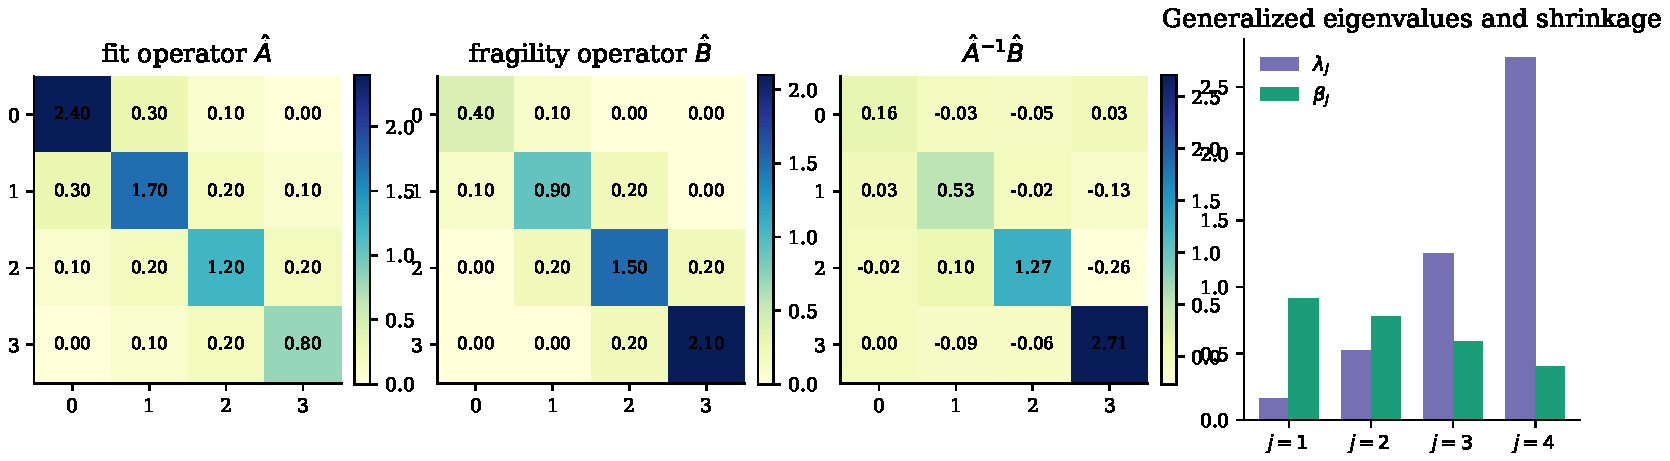
\includegraphics[width=\linewidth]{figures/operator_views.pdf}
        \caption{Inflated fit and fragility operators, their generalized geometry, and the resulting spectrum.}
        \label{fig:operators}
    \end{subfigure}
    \hfill
    \begin{subfigure}[t]{0.24\textwidth}
        \centering
        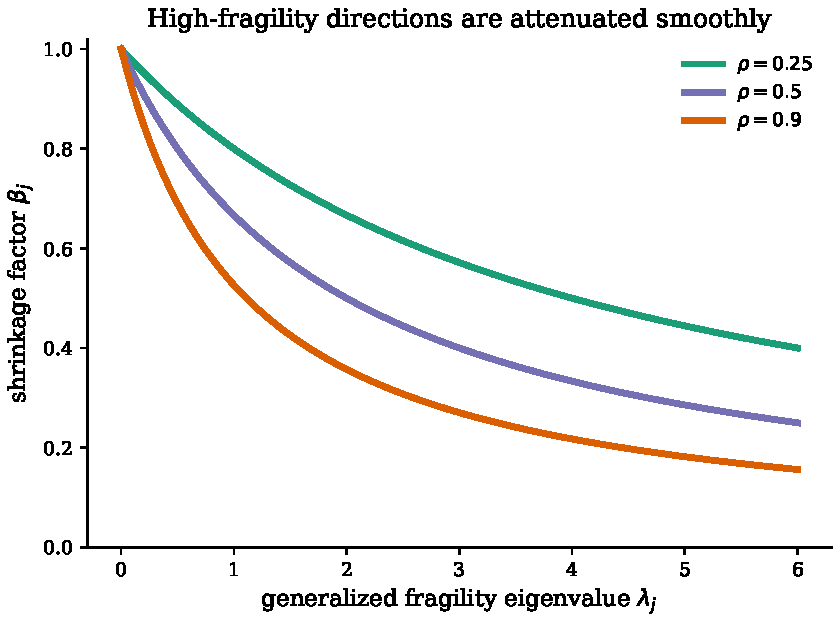
\includegraphics[width=\linewidth]{figures/shrinkage_curve.pdf}
        \caption{Shrinkage path as fragility rises.}
        \label{fig:path}
    \end{subfigure}
    \caption{\textbf{Operator-level intuition for \swing{}.} The inflated fit operator \(\hat A_\tau\) says which directions the source data trusts after isotropic certification inflation. The fragility operator \(\hat B\) says which directions swing under source-support redistributions. Their generalized eigensystem defines the contraction geometry.}
    \label{fig:operators_main}
\end{figure*}

\section{Practical Estimation Details}
\label{sec:practical}

\paragraph{Estimating the quadratic fit surrogate.}
Given local coordinates \(z_t\), projected models \(\tilde\theta_t=\mu+Uz_t\), \(t\in\cC_{\mathrm{loc}}\), and fit-split losses \(\widehat L_{\mathrm{fit}}(\tilde\theta_t)\), we estimate \((\hat c,\hat a,\hat A_0)\) by solving
\[
\min_{c,a,A_0=A_0^\top}
\sum_{t\in\cC_{\mathrm{loc}}}
\paren{
\widehat L_{\mathrm{fit}}(\tilde\theta_t)
-
c-a^\top z_t-\frac12 z_t^\top A_0 z_t
}^2
+
\eta_A \norm{A_0}_F^2
\]
subject to \(\hat A_0 \succeq m_A I_r\) for a small ridge floor \(m_A>0\). The finite-sample theory in Section~\ref{sec:theory} first analyzes the underlying unconstrained ridge fit; when the true curvature is uniformly positive definite and \(m_A\) is chosen below that population floor, the practical positivity constraint is eventually inactive. We then set \(\hat A_\tau = \hat A_0 + \tau I_r\). This makes the local source-fit surrogate strictly convex and numerically stable.
For the estimation theorems, the ridge parameters are written in normalized form, i.e. after dividing these unnormalized least-squares objectives by \(|\cC_{\mathrm{loc}}|\); this is only a rescaling convention and does not change the fitted optimizer.

\paragraph{Estimating the slope covariance.}
For each example \(Z_i \in S_{\mathrm{shift}}\), let \(\ell_{it}=\loss(\tilde\theta_t; Z_i)\). We estimate the examplewise slope vector \(\hat\phi_i\) from the local quadratic model
\[
\ell_{it}
\approx
\alpha_i + \hat\phi_i^\top z_t + \frac12 z_t^\top \hat H_i z_t,
\qquad
t\in\cC_{\mathrm{loc}},
\]
using ridge regression with penalty \(\eta_H\) over \(t\in\cC_{\mathrm{loc}}\). The fitted linear coefficient is the estimated derivative at \(z=0\). Then
\[
\hat B
=
\frac{1}{|S_{\mathrm{shift}}|}
\sum_{i\in S_{\mathrm{shift}}}
(\hat\phi_i-\bar\phi)(\hat\phi_i-\bar\phi)^\top,
\qquad
\bar\phi = \frac{1}{|S_{\mathrm{shift}}|}\sum_i \hat\phi_i.
\]
As above, the theorem-level \(\eta_H\) is the normalized version of this practical ridge penalty after dividing the per-example regression objective by \(|\cC_{\mathrm{loc}}|\).

\paragraph{Local design and identifiability.}
The quadratic fit is informative only if the local checkpoint design contains enough variation. Concretely, the design matrix formed by the intercept, the \(r\) linear monomials, and the \(\frac{r(r+1)}{2}\) unique quadratic monomials over \(\cC_{\mathrm{loc}}\) must be well conditioned; otherwise the ridge floor dominates the estimate and the recovered curvature is largely arbitrary. The same requirement applies to the per-example local quadratic regressions used to estimate \(\hat\phi_i\). These are standard local-polynomial identifiability conditions rather than consequences of split separation, and they are exactly the deterministic design conditions invoked in Assumption~\ref{ass:identify}.

\paragraph{Dimensionality versus local cloud size.}
The practical dimension of each local quadratic fit is
\[
p = 1 + r + \frac{r(r+1)}{2},
\]
so the estimator becomes statistically and numerically demanding if \(r\) is pushed too high relative to the size and diversity of \(\cC_{\mathrm{loc}}\). For example, \(r=10\) already gives \(p=66\). The intended operating regime is therefore modest rank, a local checkpoint cloud substantially richer than the raw parameter count, and explicit monitoring of design conditioning. If those conditions fail, the correct interpretation is not that \swing{} has discovered precise curvature, but that the ridge terms are forcing a conservative low-variance edit. This is exactly why the eventual empirical study must ablate \(r\), \(|\cC_{\mathrm{loc}}|\), and ridge strengths jointly.

\paragraph{Computational complexity.}
If \(d\) is the ambient parameter dimension, \(r\ll d\) is the subspace rank, \(M=|\cC|\) is the safe-pool size, and \(n_s=|S_{\mathrm{shift}}|\), then the dominant costs are:
\begin{itemize}[leftmargin=1.4em]
    \item subspace extraction from \(M\) checkpoints;
    \item one local quadratic fit in \(r\) variables for the source surrogate;
    \item batched local quadratic regressions in \(r\) variables to estimate per-example slopes;
    \item one \(r\times r\) generalized eigendecomposition.
\end{itemize}
The per-example regressions share the same local design matrix over \(\cC_{\mathrm{loc}}\). Hence the expensive linear algebra can be amortized: one factors the common ridge Gram matrix once, then applies that factorization to many example-specific right-hand sides in batch. The main remaining overhead is evaluating per-example losses over the local checkpoint cloud, which is an offline post-hoc cost on held-out source data rather than a training-time cost. This does make \swing{} materially heavier than \swad{}, but not by a factor of \(n_s\) fresh matrix factorizations.
The final deployment cost remains unchanged from ordinary single-model inference because \swing{} outputs one weight vector.

\section{Experimental Protocol}
\label{sec:experiments}

All new empirical results for \swing{} are intentionally left as \TBD{}. This section records the protocol, published benchmark context, and the exact ablations the eventual empirical study should run.

\subsection{Benchmarks and training regime}

We will evaluate on the standard DomainBed suite \citep{gulrajani2021domainbed}:
\begin{itemize}[leftmargin=1.4em]
    \item PACS,
    \item VLCS,
    \item OfficeHome,
    \item TerraIncognita,
    \item DomainNet.
\end{itemize}
The intended baseline regime is the standard ResNet-50 single-run post-hoc setting anchored by published \swad{} comparisons. EoA is included only as adjacent published context because it reports both within-run moving-average selection and heavier across-run ensemble variants. Heavier multi-run methods such as \diwa{} and ensemble variants of EoA are retained only as broader published context, not as the pure single-run reference regime. The checkpoint bank should be dense enough to resolve one late connected basin. All post-hoc selection and shrinkage must use only source-held-out data and must not use source-domain identities.

\subsection{Published benchmark context}

Table~\ref{tab:published} records exact published numbers for the main standalone baselines and direct single-model references. Table~\ref{tab:published_hybrid} then summarizes heavier averaging settings and stronger hybrid combinations. These are not new \swing{} results; they define the empirical landscape the method must eventually enter.

\begin{table}[t]
    \centering
    \small
    \begin{adjustbox}{max width=\linewidth}
    \begin{tabular}{lcccccc}
        \toprule
        Method & PACS & VLCS & OfficeHome & TerraInc. & DomainNet & Avg. \\
        \midrule
        \erm{} \citep{cha2021swad} & 85.5 & 77.5 & 66.5 & 46.1 & 40.9 & 63.3 \\
        \swad{} \citep{cha2021swad} & 88.1 & 79.1 & 70.6 & 50.0 & 46.5 & 66.9 \\
        \textsc{ERM++} \citep{teterwak2025ermpp} & 89.8 & 78.0 & 74.7 & 51.2 & 50.8 & 68.9 \\
        \bottomrule
    \end{tabular}
    \end{adjustbox}
    \caption{Standalone and direct single-model benchmark context from prior work. \textsc{ERM++} is not a post-hoc method, but it is a strong current baseline and materially raises the empirical bar.}
    \label{tab:published}
\end{table}

\begin{table}[t]
    \centering
    \small
    \begin{tabular}{lll}
        \toprule
        Setting & Method & Avg. \\
        \midrule
        Strongest EoA setting & EoA \citep{arpit2022eoa} & 68.0 \\
        Heavier multi-run post-hoc & \diwa{} \citep{rame2022diwa} & 68.0 \\
        Hybrid post-hoc & \miro{} + \swad{} \citep{cha2022miro} & 68.1 \\
        Hybrid on stronger baseline & \diwa{} + \textsc{ERM++} \citep{teterwak2025ermpp} & 69.3 \\
        Hybrid on stronger baseline & \miro{} + \textsc{ERM++} \citep{teterwak2025ermpp} & 69.4 \\
        \bottomrule
    \end{tabular}
    \caption{Heavier or hybrid benchmark context from prior work. These rows are useful reference points, but they are not the pure single-run post-hoc regime targeted by \swing{}.}
    \label{tab:published_hybrid}
\end{table}

\subsection{Planned main table}

\begin{table}[t]
    \centering
    \small
    \begin{adjustbox}{max width=\linewidth}
    \begin{tabular}{lcccccc}
        \toprule
        Method & PACS & VLCS & OfficeHome & TerraInc. & DomainNet & Avg. \\
        \midrule
        \erm{} & 85.5 & 77.5 & 66.5 & 46.1 & 40.9 & 63.3 \\
        \swad{} & 88.1 & 79.1 & 70.6 & 50.0 & 46.5 & 66.9 \\
        \textsc{ERM++} & 89.8 & 78.0 & 74.7 & 51.2 & 50.8 & 68.9 \\
        \swing{} & \TBD{} & \TBD{} & \TBD{} & \TBD{} & \TBD{} & \TBD{} \\
        \bottomrule
    \end{tabular}
    \end{adjustbox}
    \caption{Planned primary comparison in the pure single-run post-hoc regime, together with the strong standalone baseline \textsc{ERM++}. Heavier and hybrid contexts are summarized separately in Table~\ref{tab:published_hybrid}. All \swing{} entries are intentionally left as \TBD{} until experiments are run.}
    \label{tab:main_tbd}
\end{table}

\subsection{Required ablations}

The empirical study should include at least the following ablations.
\begin{enumerate}[leftmargin=1.4em]
    \item \textbf{No fragility term:} set \(B=0\) and recover the inflated baseline \(z_\tau\).
    \item \textbf{Scalar shrinkage:} replace generalized shrinkage with the best one-parameter interpolation toward \(\mu\).
    \item \textbf{No safe pool:} build \(U\) from a broader late trajectory without the barrier screen.
    \item \textbf{Rank sensitivity:} vary \(r\).
    \item \textbf{Local-cloud sensitivity:} vary \(|\cC_{\mathrm{loc}}|\) or \(\rho_{\mathrm{loc}}\), and report the resulting design conditioning.
    \item \textbf{Regularization sensitivity:} vary \(\lambda\) and the ridge strengths \((\eta_A,\eta_H)\).
    \item \textbf{Inflation sensitivity:} vary \(\tau\).
    \item \textbf{Split overlap test:} compare disjoint versus reused fit/shift splits.
\end{enumerate}

\begin{table}[t]
    \centering
    \small
    \begin{tabular}{lc}
        \toprule
        Variant & Avg. Acc. \\
        \midrule
        \swing{} & \TBD{} \\
        No fragility term (\(B=0\)) & \TBD{} \\
        Best scalar shrinkage & \TBD{} \\
        No safe pool screen & \TBD{} \\
        Small rank \(r\) & \TBD{} \\
        Large rank \(r\) & \TBD{} \\
        Small \(\lambda\) & \TBD{} \\
        Large \(\lambda\) & \TBD{} \\
        Small \(\tau\) & \TBD{} \\
        Large \(\tau\) & \TBD{} \\
        \bottomrule
    \end{tabular}
    \caption{Planned ablation table. All new numbers remain \TBD{}.}
    \label{tab:ablations_tbd}
\end{table}

\section{Discussion}

\paragraph{What \swing{} is and is not.}
\swing{} is not another global soup optimizer. It is also not a last-layer repair method, not a multi-run averaging scheme, and not a target-time adaptation method. It is a full-weight basin edit that acts only after a safe post-hoc basin has already been found.

\paragraph{Why the theory is local.}
The paper's theory is intentionally restricted to a connected low-rank basin family. That is a strength, not a weakness. The whole operational point of post-hoc single-run DG is that one dense trajectory often already contains a safe region; the scientifically honest question is what can be proved \emph{inside that region}.

\paragraph{Limitations.}
The theory assumes a source-supported local shift model. If the target domain introduces genuinely new support, novel backgrounds, or unsupported feature mechanisms, then source-reweighting fragility cannot fully characterize deployment risk; this is a structural limitation of source-only post-hoc methods rather than a hidden claim of the paper. The quadratic source-fit model is also local, and the regression estimators for \(A_0\) and \(B\) can become noisy if the safe pool is too small or too narrow or if the local design is poorly conditioned. Because the local polynomial dimension scales as \(1+r+r(r+1)/2\), high-rank fits require correspondingly richer checkpoint clouds; otherwise ridge regularization will dominate and the edit will become conservative. The certificate interpretation should also be read in forward form: a chosen \(\tau\) certifies only local source-supported shifts with radius \(\varrho \le (\tau/K)^2\). Finally, the eventual empirical study must verify that the gains are not captured by simpler scalar shrinkage, by isotropic inflation alone, or by aggressive ridge settings that wash out the intended geometry.

\section{Conclusion}

\swing{} is a simple claim made operational: once a good checkpoint basin has been found, not all directions inside that basin should be trusted equally. Directions whose contribution swings under plausible source-support reweightings should be shrunk. The resulting method stays single-run, post-hoc, domain-label-free, and single-model at test time. Its math is now explicit end to end: barrier filtering yields a population-safe star pool up to concentration margins; bounded negative curvature makes averaging inside that filtered basin safe up to an explicit variance term; a hidden-shift upper bound yields a square-root fragility term and an exact minimax/dual interpretation; the inflated surrogate admits generalized eigen-shrinkage and a quantitative scalar-gap theorem; and the deployed constrained estimator enjoys finite-sample control once the local operators are estimated accurately. The empirical study remains to be run; the paper, figures, proofs, and protocol are ready.

\bibliographystyle{plainnat}
\bibliography{references}

\appendix

\section{Additional Geometric Intuition}

\begin{figure}[H]
    \centering
    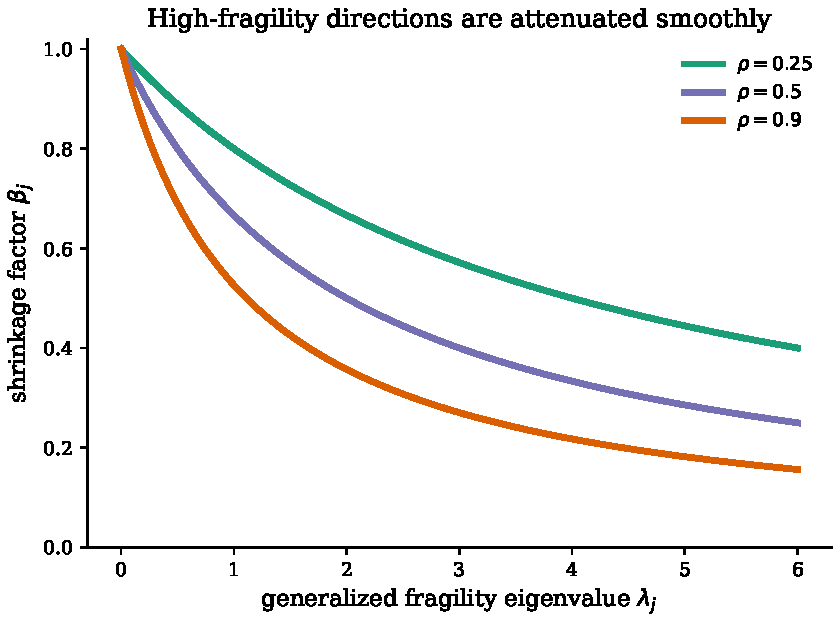
\includegraphics[width=0.7\linewidth]{figures/shrinkage_curve.pdf}
    \caption{\textbf{Regularization path.} Each generalized direction is shrunk by \(\beta_j(\lambda)=1/(1+\lambda\nu_j)\). Larger fragility eigenvalues decay faster as \(\lambda\) grows.}
    \label{fig:path_appendix}
\end{figure}

\section{Proofs}

\subsection{Proof of Theorem~\ref{thm:pool_filter}}

\begin{proof}
\(\widehat L_{\mathrm{pool}}(\theta)\) is the empirical average of the bounded loss at model \(\theta\) over \(S_{\mathrm{pool}}\). For each checkpoint \(t\in[T]\) and each ordered interpolation model \((1-\alpha)\theta_i+\alpha\theta_j\) with \((i,j,\alpha)\in[T]\times[T]\times\mathcal G\), Hoeffding's inequality gives
\[
\Pr\!\paren{
\abs{\widehat L_{\mathrm{pool}}(\theta_t)-L_P(\theta_t)} > \xi
}
\le
2\exp\!\paren{
-\frac{2\abs{S_{\mathrm{pool}}}\xi^2}{(L_{\max}^{\mathrm{pool}})^2}
},
\]
\[
\Pr\!\paren{
\abs{\widehat L_{\mathrm{pool}}\!\paren{(1-\alpha)\theta_i+\alpha\theta_j} - L_P\!\paren{(1-\alpha)\theta_i+\alpha\theta_j}} > \xi
}
\le
2\exp\!\paren{
-\frac{2\abs{S_{\mathrm{pool}}}\xi^2}{(L_{\max}^{\mathrm{pool}})^2}
}.
\]
There are \(T\) checkpoint models and \(T^2\abs{\mathcal G}\) ordered interpolation models. Hence, by the union bound, with probability at least \(1-\delta\), the event
\[
\mathcal E_{\mathrm{pool}}
:=
\Bigl\{
\sup_{1\le t\le T}\abs{\widehat L_{\mathrm{pool}}(\theta_t)-L_P(\theta_t)}\le \xi_{\mathrm{pool}}(\delta),\
\sup_{\substack{1\le i,j\le T\\ \alpha\in\mathcal G}}
\abs{
\widehat L_{\mathrm{pool}}\!\paren{(1-\alpha)\theta_i+\alpha\theta_j}
-
L_P\!\paren{(1-\alpha)\theta_i+\alpha\theta_j}
}
\le \xi_{\mathrm{pool}}(\delta)
\Bigr\}
\]
holds.

Work on \(\mathcal E_{\mathrm{pool}}\). Let \(t^\star\in\argmin_{1\le t\le T} L_P(\theta_t)\). Since \(a\) minimizes the empirical checkpoint risk,
\[
\widehat L_{\mathrm{pool}}(\theta_a)\le \widehat L_{\mathrm{pool}}(\theta_{t^\star}).
\]
Therefore
\[
L_P(\theta_a)
\le
\widehat L_{\mathrm{pool}}(\theta_a) + \xi_{\mathrm{pool}}(\delta)
\le
\widehat L_{\mathrm{pool}}(\theta_{t^\star}) + \xi_{\mathrm{pool}}(\delta)
\le
L_P(\theta_{t^\star}) + 2\xi_{\mathrm{pool}}(\delta),
\]
which proves the anchor bound.

Now fix \(t\in\cC\). By definition of the empirical pool,
\[
\widehat L_{\mathrm{pool}}(\theta_t)
\le
\widehat L_{\mathrm{pool}}(\theta_a) + \varepsilon_{\mathrm{pool}}.
\]
Hence
\[
L_P(\theta_t)
\le
\widehat L_{\mathrm{pool}}(\theta_t) + \xi_{\mathrm{pool}}(\delta)
\le
\widehat L_{\mathrm{pool}}(\theta_a) + \varepsilon_{\mathrm{pool}} + \xi_{\mathrm{pool}}(\delta)
\le
L_P(\theta_a) + \varepsilon_{\mathrm{pool}} + 2\xi_{\mathrm{pool}}(\delta).
\]
Likewise, the empirical barrier condition for \(t\in\cC\) gives
\[
\max_{\alpha\in\mathcal G}
\widehat L_{\mathrm{pool}}\!\paren{(1-\alpha)\theta_a+\alpha\theta_t}
\le
\max\braces{\widehat L_{\mathrm{pool}}(\theta_a),\widehat L_{\mathrm{pool}}(\theta_t)}
+
\tau_{\mathrm{pool}}.
\]
For each fixed \(\alpha\in\mathcal G\), event \(\mathcal E_{\mathrm{pool}}\) implies
\begin{align*}
L_P\!\paren{(1-\alpha)\theta_a+\alpha\theta_t}
&\le
\widehat L_{\mathrm{pool}}\!\paren{(1-\alpha)\theta_a+\alpha\theta_t}
+
\xi_{\mathrm{pool}}(\delta) \\
&\le
\max\braces{\widehat L_{\mathrm{pool}}(\theta_a),\widehat L_{\mathrm{pool}}(\theta_t)}
+
\tau_{\mathrm{pool}}
+
\xi_{\mathrm{pool}}(\delta) \\
&\le
\max\braces{L_P(\theta_a),L_P(\theta_t)}
+
\tau_{\mathrm{pool}}
+
2\xi_{\mathrm{pool}}(\delta).
\end{align*}
Taking the maximum over \(\alpha\in\mathcal G\) proves the grid-barrier claim.
\end{proof}

\subsection{Proof of Corollary~\ref{cor:segment_barrier}}

\begin{proof}
Fix \(t\in\cC\). Define
\[
g_t(u) = L_P\!\paren{(1-u)\theta_a + u\theta_t},
\qquad
u\in[0,1].
\]
Because \(L_P\) is differentiable on \(\mathfrak S_a(\cC)\), \(g_t\) is differentiable on \([0,1]\) with derivative
\[
g_t'(u)
=
\nabla L_P\!\paren{(1-u)\theta_a+u\theta_t}^\top (\theta_t-\theta_a).
\]
Hence
\[
\abs{g_t'(u)}
\le
G_{\mathrm{pool}}\norm{\theta_t-\theta_a}
\qquad
\text{for all } u\in[0,1].
\]
Let \(u\in[0,1]\). By definition of \(\gamma(\mathcal G)\), choose \(\alpha_u\in\mathcal G\) such that \(\abs{u-\alpha_u}\le \gamma(\mathcal G)\). The mean-value theorem yields
\[
\abs{g_t(u)-g_t(\alpha_u)}
\le
G_{\mathrm{pool}}\norm{\theta_t-\theta_a}\,\gamma(\mathcal G).
\]
Therefore
\begin{align*}
g_t(u)
&\le
g_t(\alpha_u) + G_{\mathrm{pool}}\norm{\theta_t-\theta_a}\,\gamma(\mathcal G) \\
&\le
\max\braces{L_P(\theta_a),L_P(\theta_t)}
+
\tau_{\mathrm{pool}}
+
2\xi_{\mathrm{pool}}(\delta)
+
G_{\mathrm{pool}}\norm{\theta_t-\theta_a}\,\gamma(\mathcal G),
\end{align*}
where the second inequality is Theorem~\ref{thm:pool_filter}. Taking the supremum over \(u\in[0,1]\) proves the claim.
\end{proof}

\subsection{Proof of Theorem~\ref{thm:soup_safe}}

\begin{proof}
Fix any \(t\in\cC\). Taylor's theorem around \(\theta_w\) gives
\[
L_P(\theta_t)
=
L_P(\theta_w)
+
\nabla L_P(\theta_w)^\top (\theta_t-\theta_w)
+
\frac12 (\theta_t-\theta_w)^\top \nabla^2 L_P(\tilde\theta_t)(\theta_t-\theta_w)
\]
for some \(\tilde\theta_t\) on the segment joining \(\theta_w\) and \(\theta_t\), hence inside \(\operatorname{conv}(\cC)\). Since \(\nabla^2 L_P(\tilde\theta_t)\succeq -\beta_{\mathrm{pool}}I_d\),
\[
L_P(\theta_t)
\ge
L_P(\theta_w)
+
\nabla L_P(\theta_w)^\top (\theta_t-\theta_w)
-
\frac{\beta_{\mathrm{pool}}}{2}\norm{\theta_t-\theta_w}^2.
\]
Multiply by \(w_t\) and sum over \(t\in\cC\):
\[
\sum_{t\in\cC} w_t L_P(\theta_t)
\ge
L_P(\theta_w)
+
\nabla L_P(\theta_w)^\top \sum_{t\in\cC} w_t(\theta_t-\theta_w)
-
\frac{\beta_{\mathrm{pool}}}{2}
\sum_{t\in\cC} w_t \norm{\theta_t-\theta_w}^2.
\]
Because \(\theta_w=\sum_{t\in\cC} w_t\theta_t\), the middle term vanishes. Rearranging gives
\[
L_P(\theta_w)
\le
\sum_{t\in\cC} w_t L_P(\theta_t)
+
\frac{\beta_{\mathrm{pool}}}{2}
\sum_{t\in\cC} w_t \norm{\theta_t-\theta_w}^2.
\]
If every \(t\in\cC\) satisfies \(L_P(\theta_t)\le L_P(\theta_a)+\varepsilon_{\mathrm{safe}}\), then
\[
\sum_{t\in\cC} w_t L_P(\theta_t)\le L_P(\theta_a)+\varepsilon_{\mathrm{safe}},
\]
and substituting this into the previous display proves the second bound.
\end{proof}

\subsection{Proof of Theorem~\ref{thm:robust_bound}}

\begin{proof}
Fix \(z\in\cZ\) and \(Q\in\cQ(\varrho)\). By Assumption~\ref{ass:shift}, there exists \(h\) such that \(dQ/dP = 1+h\), \(\EE_P[h]=0\), and \(\EE_P[h^2]\le \varrho\). Therefore
\begin{align}
L_Q(z)-L_Q(0)
&=
\EE_Q\bracks{\loss(\theta(z);Z)-\loss(\theta(0);Z)} \notag\\
&=
\EE_P\bracks{(1+h(Z))\paren{\loss(\theta(z);Z)-\loss(\theta(0);Z)}}.
\label{eq:proof_t1_start}
\end{align}
By Assumption~\ref{ass:lin},
\[
\loss(\theta(z);Z)
=
\loss(\theta(0);Z)
+
\phi(Z)^\top z
+
r(Z,z).
\]
Substituting this into \eqref{eq:proof_t1_start} gives
\begin{align}
L_Q(z)-L_Q(0)
&=
\EE_P\bracks{\phi(Z)^\top z}
+
\EE_P\bracks{r(Z,z)}
+
\EE_P\bracks{h(Z)\phi(Z)^\top z}
+
\EE_P\bracks{h(Z)r(Z,z)}.
\label{eq:proof_t1_expand}
\end{align}
Write \(\bar\phi=\EE_P[\phi(Z)]\). Since \(\EE_P[h]=0\),
\[
\EE_P\bracks{h(Z)\phi(Z)^\top z}
=
\EE_P\bracks{h(Z)(\phi(Z)-\bar\phi)^\top z}.
\]
Apply Cauchy--Schwarz:
\begin{align}
\abs{\EE_P\bracks{h(Z)(\phi(Z)-\bar\phi)^\top z}}
&\le
\sqrt{\EE_P[h(Z)^2]}
\sqrt{\EE_P\bracks{\paren{(\phi(Z)-\bar\phi)^\top z}^2}} \notag\\
&\le
\sqrt{\varrho}
\sqrt{z^\top \EE_P\bracks{(\phi(Z)-\bar\phi)(\phi(Z)-\bar\phi)^\top} z} \notag\\
&=
\sqrt{\varrho\, z^\top B z}.
\label{eq:proof_t1_phi}
\end{align}
Next, use the remainder bound from Assumption~\ref{ass:lin},
\[
\abs{r(Z,z)} \le \frac{\kappa(Z)}{2}\norm{z}^2.
\]
Applying Cauchy--Schwarz again,
\begin{align}
\abs{\EE_P\bracks{h(Z)r(Z,z)}}
&\le
\sqrt{\EE_P[h(Z)^2]}
\sqrt{\EE_P[r(Z,z)^2]} \notag\\
&\le
\sqrt{\varrho}
\sqrt{
\EE_P\bracks{\frac{\kappa(Z)^2}{4}\norm{z}^4}
} \notag\\
&=
\frac{\sqrt{\varrho}}{2}\norm{z}^2
\sqrt{\EE_P[\kappa(Z)^2]} \notag\\
&\le
\frac{\sqrt{\varrho}\,K}{2}\norm{z}^2.
\label{eq:proof_t1_remainder}
\end{align}
Finally, by Assumption~\ref{ass:fit},
\[
L_P(z)-L_P(0)=a^\top z + \frac12 z^\top A_0 z.
\]
The first two terms on the right-hand side of \eqref{eq:proof_t1_expand} therefore combine to
\[
\EE_P\bracks{\phi(Z)^\top z}
+
\EE_P\bracks{r(Z,z)}
=
L_P(z)-L_P(0)
=
a^\top z + \frac12 z^\top A_0 z.
\]
Combining this identity with \eqref{eq:proof_t1_expand}, \eqref{eq:proof_t1_phi}, and \eqref{eq:proof_t1_remainder} yields
\[
L_Q(z)-L_Q(0)
\le
a^\top z + \frac12 z^\top A_0 z
+
\sqrt{\varrho\, z^\top B z}
+
\frac{\sqrt{\varrho}\,K}{2}\norm{z}^2.
\]
Adding \(L_Q(0)\) to both sides gives the claimed inequality.
\end{proof}

\subsection{Proof of Corollary~\ref{cor:quadratic_majorizer}}

\begin{proof}
Start from Theorem~\ref{thm:robust_bound}:
\[
L_Q(z)
\le
L_Q(0)
+
a^\top z + \frac12 z^\top A_0 z
+
\sqrt{\varrho\, z^\top B z}
+
\frac{\sqrt{\varrho}\,K}{2}\norm{z}^2.
\]
For any \(\lambda>0\) and any \(u\ge 0\), Young's inequality gives
\[
\sqrt{\varrho\,u}
\le
\frac{\varrho}{2\lambda} + \frac{\lambda}{2}u.
\]
Apply this with \(u=z^\top B z\) to obtain
\[
\sqrt{\varrho\, z^\top B z}
\le
\frac{\varrho}{2\lambda}
+
\frac{\lambda}{2} z^\top B z.
\]
Also,
\[
\frac12 z^\top A_0 z + \frac{\sqrt{\varrho}\,K}{2}\norm{z}^2
\le
\frac12 z^\top \paren{A_0 + \tau I_r}z
=
\frac12 z^\top A_\tau z,
\]
where the inequality uses \(\tau\ge \sqrt{\varrho}K\). Substituting both inequalities into the bound from Theorem~\ref{thm:robust_bound} yields
\[
L_Q(z)
\le
L_Q(0) + \frac{\varrho}{2\lambda}
+
a^\top z
+
\frac12 z^\top A_\tau z
+
\frac{\lambda}{2} z^\top B z.
\]
This is the desired claim.
\end{proof}

\subsection{Proof of Proposition~\ref{prop:minimax}}

\begin{proof}
For fixed \(z\), the Euclidean support-function identity gives
\[
\sup_{\norm{u}_2\le \sqrt{\varrho}} u^\top B^{1/2}z
=
\sqrt{\varrho}\,\norm{B^{1/2}z}_2
=
\sqrt{\varrho\, z^\top B z}.
\]
Adding the deterministic term \(a^\top z + \frac12 z^\top A_\tau z\) yields the first representation.

For the second representation, fix \(u=z^\top B z\ge 0\) and consider
\[
\psi_u(\lambda)=\frac{\varrho}{2\lambda} + \frac{\lambda}{2}u,
\qquad \lambda>0.
\]
If \(u>0\), then \(\psi_u'(\lambda) = -\frac{\varrho}{2\lambda^2} + \frac{u}{2}\), so the unique minimizer is \(\lambda^\star=\sqrt{\varrho/u}\), with
\[
\psi_u(\lambda^\star)=\sqrt{\varrho u}.
\]
If \(u=0\), then \(\psi_u(\lambda)=\varrho/(2\lambda)\), so \(\inf_{\lambda>0}\psi_u(\lambda)=0=\sqrt{\varrho u}\). Consequently
\[
\sqrt{\varrho\, z^\top B z}
=
\inf_{\lambda>0}
\bracks{
\frac{\varrho}{2\lambda} + \frac{\lambda}{2}z^\top B z
}.
\]
Adding \(a^\top z + \frac12 z^\top A_\tau z\) proves the second representation.
\end{proof}

\subsection{Proof of Theorem~\ref{thm:closed_form}}

\begin{proof}
Because \(A_\tau\succ 0\) and \(B\succeq 0\), the matrix \(A_\tau+\lambda B\) is positive definite for every \(\lambda>0\). Hence the quadratic function
\[
J_{\lambda,\tau}(z)=a^\top z + \frac12 z^\top A_\tau z + \frac{\lambda}{2} z^\top B z
\]
is strongly convex and has a unique minimizer. Its gradient is
\[
\nabla J_{\lambda,\tau}(z)=a + A_\tau z + \lambda Bz.
\]
Setting the gradient equal to zero yields the normal equation
\[
(A_\tau+\lambda B)z = -a.
\]
Therefore
\[
z_{\lambda,\tau}^{\mathrm{unc}} = -(A_\tau+\lambda B)^{-1}a.
\]
Because \(z_\tau=-A_\tau^{-1}a\), we may rewrite this as
\[
z_{\lambda,\tau}^{\mathrm{unc}} = (A_\tau+\lambda B)^{-1}A_\tau z_\tau.
\]
This proves the first claim.

Because \(A_\tau\succ 0\) and \(B\succeq 0\), the symmetric generalized eigenproblem admits an \(A_\tau\)-orthonormal basis \(V=[v_1,\dots,v_r]\) and nonnegative eigenvalues \(\nu_1,\dots,\nu_r\) satisfying
\[
BV = A_\tau V \diag(\nu_1,\dots,\nu_r),
\qquad
V^\top A_\tau V = I.
\]
Expand
\[
z_\tau = Vc,
\qquad
c = V^\top A_\tau z_\tau.
\]
If \(z=Vy\), then
\begin{align}
J_{\lambda,\tau}(Vy)
&=
a^\top Vy + \frac12 y^\top V^\top A_\tau V y + \frac{\lambda}{2} y^\top V^\top B V y \notag\\
&=
a^\top Vy + \frac12 y^\top y + \frac{\lambda}{2} y^\top \diag(\nu_1,\dots,\nu_r) y.
\label{eq:proof_closed_coord}
\end{align}
Using \(a=-A_\tau z_\tau=-A_\tau Vc\), we obtain
\[
a^\top Vy = -c^\top y.
\]
Substituting this into \eqref{eq:proof_closed_coord} gives
\[
J_{\lambda,\tau}(Vy)
=
\sum_{j=1}^r\bracks{-c_j y_j + \frac12 (1+\lambda\nu_j)y_j^2}.
\]
The coordinates decouple, and each one is minimized at \(y_j=c_j/(1+\lambda\nu_j)\). Therefore
\[
z_{\lambda,\tau}^{\mathrm{unc}}
=
\sum_{j=1}^r \frac{c_j}{1+\lambda\nu_j}v_j.
\]
If \(z_{\lambda,\tau}^{\mathrm{unc}}\in\cZ\), then it is also the constrained minimizer because the constrained and unconstrained problems share the same objective and \(\cZ\) contains the unconstrained optimum.
\end{proof}

\subsection{Proof of Proposition~\ref{prop:scalar_gap}}

\begin{proof}
If \(z_\tau=0\), then \(\mathcal F_{\mathrm{sc}}=\{0\}\) and Theorem~\ref{thm:closed_form} gives \(z_{\lambda,\tau}^{\mathrm{unc}}=0\), so the gap is zero. Assume now that \(z_\tau\neq 0\), hence \(S=\sum_j c_j^2>0\).

For scalar shrinkage,
\[
J_{\lambda,\tau}(\alpha z_\tau)
=
\sum_{j=1}^r\bracks{-\alpha c_j^2 + \frac12 (1+\lambda\nu_j)\alpha^2 c_j^2}
=
\frac{S}{2}\bracks{-2\alpha + \alpha^2\paren{1+\lambda\sum_{j=1}^r p_j\nu_j}}.
\]
The minimizing scalar is therefore
\[
\alpha^\star
=
\frac{1}{1+\lambda\sum_{j=1}^r p_j\nu_j}
=
f_\lambda\!\paren{\sum_{j=1}^r p_j\nu_j},
\]
and the corresponding objective value is
\[
\min_{\alpha\in\RR}J_{\lambda,\tau}(\alpha z_\tau)
=
-\frac{S}{2}
f_\lambda\!\paren{\sum_{j=1}^r p_j\nu_j}.
\]
By Theorem~\ref{thm:closed_form},
\[
J_{\lambda,\tau}(z_{\lambda,\tau}^{\mathrm{unc}})
=
\sum_{j=1}^r\bracks{
-\frac{c_j^2}{1+\lambda\nu_j}
+
\frac12 (1+\lambda\nu_j)\frac{c_j^2}{(1+\lambda\nu_j)^2}
}
=
-\frac12\sum_{j=1}^r \frac{c_j^2}{1+\lambda\nu_j}
=
-\frac{S}{2}\sum_{j=1}^r p_j f_\lambda(\nu_j).
\]
Subtracting the two identities yields
\[
\Delta_{\mathrm{sc}}
=
\frac{S}{2}
\bracks{
\sum_{j=1}^r p_j f_\lambda(\nu_j)
-
f_\lambda\!\paren{\sum_{j=1}^r p_j\nu_j}
}.
\]
Since
\[
f_\lambda''(\nu)=\frac{2\lambda^2}{(1+\lambda\nu)^3}>0,
\]
\(f_\lambda\) is convex on \([0,\infty)\), so Jensen's inequality implies \(\Delta_{\mathrm{sc}}\ge 0\). Equality in Jensen's inequality holds if and only if the active generalized eigenvalues are constant, that is, if and only if \(\nu_j\) is constant on the support of \(z_\tau\).

For the variance lower bound, let \(\bar\nu=\sum_j p_j\nu_j\). Taylor's theorem around \(\bar\nu\) gives, for every \(x\in[0,\nu_{\max}^{\mathrm{act}}]\),
\[
f_\lambda(x)
\ge
f_\lambda(\bar\nu)
+
f_\lambda'(\bar\nu)(x-\bar\nu)
+
\frac12 \inf_{0\le s\le \nu_{\max}^{\mathrm{act}}} f_\lambda''(s)\,(x-\bar\nu)^2.
\]
Since \(f_\lambda''\) is decreasing,
\[
\inf_{0\le s\le \nu_{\max}^{\mathrm{act}}} f_\lambda''(s)
=
\frac{2\lambda^2}{(1+\lambda\nu_{\max}^{\mathrm{act}})^3}.
\]
Averaging under the weights \(p_j\) annihilates the linear term and yields
\[
\sum_{j=1}^r p_j f_\lambda(\nu_j) - f_\lambda(\bar\nu)
\ge
\frac{\lambda^2}{(1+\lambda\nu_{\max}^{\mathrm{act}})^3}\Var_p(\nu).
\]
Multiplying by \(S/2\) proves the displayed lower bound for \(\Delta_{\mathrm{sc}}\).
\end{proof}

\subsection{Proof of Proposition~\ref{prop:gain}}

\begin{proof}
Because \(z_{\lambda,\tau}^{\mathrm{unc}}\) is the minimizer of the quadratic \(J_{\lambda,\tau}\), the completion-of-squares identity yields
\[
J_{\lambda,\tau}(z)
=
J_{\lambda,\tau}(z_{\lambda,\tau}^{\mathrm{unc}})
+
\frac12 (z-z_{\lambda,\tau}^{\mathrm{unc}})^\top (A_\tau+\lambda B)(z-z_{\lambda,\tau}^{\mathrm{unc}})
\qquad
\text{for all } z\in\RR^r.
\]
Applying this with \(z=z_\tau\) gives
\[
J_{\lambda,\tau}(z_\tau) - J_{\lambda,\tau}(z_{\lambda,\tau}^{\mathrm{unc}})
=
\frac12 (z_\tau-z_{\lambda,\tau}^{\mathrm{unc}})^\top (A_\tau+\lambda B)(z_\tau-z_{\lambda,\tau}^{\mathrm{unc}}).
\]
Because \(A_\tau+\lambda B\succ 0\), the right-hand side is nonnegative, so \(J_{\lambda,\tau}(z_{\lambda,\tau}^{\mathrm{unc}})\le J_{\lambda,\tau}(z_\tau)\).

Equality holds if and only if \(z_\tau=z_{\lambda,\tau}^{\mathrm{unc}}\). By Theorem~\ref{thm:closed_form},
\[
z_{\lambda,\tau}^{\mathrm{unc}}=(A_\tau+\lambda B)^{-1}A_\tau z_\tau.
\]
Thus equality is equivalent to
\[
(A_\tau+\lambda B)z_\tau = A_\tau z_\tau,
\]
which reduces to \(\lambda Bz_\tau=0\), hence to \(Bz_\tau=0\).
\end{proof}

\subsection{Proof of Theorem~\ref{thm:constrained}}

\begin{proof}
Let
\[
\Delta = \hat z_{\lambda,\tau}^{\cZ} - z_{\lambda,\tau}^{\cZ}.
\]
Since \(z_{\lambda,\tau}^{\cZ}\) minimizes \(z\mapsto a^\top z + \frac12 z^\top M z\) over the compact convex set \(\cZ\), the variational inequality for convex optimization gives
\[
\ip{a+Mz_{\lambda,\tau}^{\cZ}}{z-z_{\lambda,\tau}^{\cZ}} \ge 0
\qquad
\text{for all } z\in\cZ.
\]
Evaluating at \(z=\hat z_{\lambda,\tau}^{\cZ}\) yields
\[
\ip{a+Mz_{\lambda,\tau}^{\cZ}}{\Delta} \ge 0.
\]
Likewise, optimality of \(\hat z_{\lambda,\tau}^{\cZ}\) gives
\[
\ip{\hat a+\hat M\hat z_{\lambda,\tau}^{\cZ}}{z-\hat z_{\lambda,\tau}^{\cZ}} \ge 0
\qquad
\text{for all } z\in\cZ.
\]
Evaluating at \(z=z_{\lambda,\tau}^{\cZ}\) yields
\[
\ip{\hat a+\hat M\hat z_{\lambda,\tau}^{\cZ}}{-\Delta}\ge 0,
\qquad\text{equivalently}\qquad
\ip{\hat a+\hat M\hat z_{\lambda,\tau}^{\cZ}}{\Delta}\le 0.
\]
Subtracting the second inequality from the first gives
\[
\ip{a-\hat a + Mz_{\lambda,\tau}^{\cZ}-\hat M\hat z_{\lambda,\tau}^{\cZ}}{\Delta}\ge 0.
\]
Since
\[
Mz_{\lambda,\tau}^{\cZ}-\hat M\hat z_{\lambda,\tau}^{\cZ}
=
-M\Delta - (\hat M-M)\hat z_{\lambda,\tau}^{\cZ},
\]
we obtain
\[
\ip{M\Delta}{\Delta}
\le
\ip{a-\hat a - (\hat M-M)\hat z_{\lambda,\tau}^{\cZ}}{\Delta}.
\]
The left-hand side is bounded below by \(m\norm{\Delta}^2\). For the right-hand side,
\[
\abs{\ip{a-\hat a - (\hat M-M)\hat z_{\lambda,\tau}^{\cZ}}{\Delta}}
\le
\paren{\norm{\hat a-a} + \norm{\hat M-M}\,\norm{\hat z_{\lambda,\tau}^{\cZ}}}\norm{\Delta}.
\]
Because \(\hat z_{\lambda,\tau}^{\cZ}\in\cZ\), \(\norm{\hat z_{\lambda,\tau}^{\cZ}}\le D_\cZ\), and because \(\norm{\hat M-M}\le \delta\),
\[
m\norm{\Delta}^2
\le
\paren{\norm{\hat a-a} + D_\cZ\delta}\norm{\Delta}.
\]
If \(\Delta=0\), the claim is immediate. Otherwise divide by \(\norm{\Delta}\) to obtain
\[
\norm{\hat z_{\lambda,\tau}^{\cZ} - z_{\lambda,\tau}^{\cZ}}
\le
\frac{\norm{\hat a-a} + D_\cZ\delta}{m}.
\]
\end{proof}

\subsection{Proof of Theorem~\ref{thm:A_est}}

\begin{proof}
Let \(N_f=\abs{S_{\mathrm{fit},n}}\). Define the response vector
\[
\hat y_n \in \RR^{m_n},
\qquad
(\hat y_n)_t = \widehat L_{\mathrm{fit}}(\tilde\theta_t)
=
\frac{1}{N_f}\sum_{i=1}^{N_f} \loss(\tilde\theta_t;Z_i),
\]
and its population counterpart
\[
y_n \in \RR^{m_n},
\qquad
(y_n)_t = L_P(z_t).
\]
By Assumption~\ref{ass:fit}, \(y_n = X_n\beta_0\). Define the normalized ridge objective
\[
Q_n(\beta)
=
\frac{1}{m_n}\norm{\hat y_n - X_n\beta}_2^2 + \eta_{A,n}\norm{P_A\beta}_2^2.
\]
Its minimizer \(\tilde\beta_n\) satisfies the normal equations
\[
(G_n+\eta_{A,n}P_A)\tilde\beta_n = \frac{1}{m_n}X_n^\top \hat y_n.
\]
Subtracting \((G_n+\eta_{A,n}P_A)\beta_0 = \frac{1}{m_n}X_n^\top y_n + \eta_{A,n}P_A\beta_0\) yields
\[
(G_n+\eta_{A,n}P_A)(\tilde\beta_n-\beta_0)
=
\frac{1}{m_n}X_n^\top(\hat y_n-y_n) - \eta_{A,n}P_A\beta_0.
\]
Since \(\lambda_{\min}(G_n)\ge \kappa_A\),
\[
\norm{(G_n+\eta_{A,n}P_A)^{-1}}_{\mathrm{op}}
\le
\frac{1}{\kappa_A}.
\]
Therefore
\[
\norm{\tilde\beta_n-\beta_0}_2
\le
\frac{
\norm{\frac{1}{m_n}X_n^\top(\hat y_n-y_n)}_2 + \eta_{A,n}\norm{P_A\beta_0}_2
}{\kappa_A}.
\]
For each fit example \(Z_i\), define
\[
\zeta_i
=
\frac{1}{m_n}\sum_{t\in\cC_{\mathrm{loc},n}}
\psi(z_t)\paren{\loss(\tilde\theta_t;Z_i)-L_P(z_t)}
\in \RR^p.
\]
Then \(\EE[\zeta_i]=0\) and
\[
\frac{1}{m_n}X_n^\top(\hat y_n-y_n)
=
\frac{1}{N_f}\sum_{i=1}^{N_f}\zeta_i.
\]
For each coordinate \(k\in[p]\),
\[
\abs{(\zeta_i)_k}
\le
\frac{1}{m_n}\sum_{t\in\cC_{\mathrm{loc},n}}
\abs{\psi_k(z_t)}\,\abs{\loss(\tilde\theta_t;Z_i)-L_P(z_t)}
\le
M_{\psi,n}L_{\max}^{\mathrm{fit}}.
\]
Hoeffding's inequality and a union bound over the \(p\) coordinates imply that, with probability at least \(1-\delta\),
\[
\norm{\frac{1}{N_f}\sum_{i=1}^{N_f}\zeta_i}_2
\le
\sqrt{p}\,M_{\psi,n}L_{\max}^{\mathrm{fit}}
\sqrt{\frac{\log(2p/\delta)}{2N_f}}.
\]
Substituting this into the previous deterministic inequality proves the bound for \(\tilde\beta_n\).

If the practical positivity floor is inactive, then the implemented estimator equals the unconstrained ridge estimator, so the same bound applies. The final displayed inequality follows because the maps \(\beta\mapsto a\) and \(\beta\mapsto A_0\) are fixed linear unpacking maps whose operator norms depend only on \(r\).
\end{proof}

\subsection{Proof of Theorem~\ref{thm:B_est}}

\begin{proof}
Let \(Z_i\in S_{\mathrm{shift},n}\) be fixed. By Assumption~\ref{ass:identify}, the examplewise loss \(g_i(z)=\loss(\theta(z);Z_i)\) is three times continuously differentiable near \(0\). Its second-order Taylor expansion at \(0\) can be written as
\[
g_i(z)=\beta(Z_i)^\top \psi(z) + r_i(z),
\]
where the linear block of \(\beta(Z_i)\) is \(\phi(Z_i)\) and
\[
\abs{r_i(z)}
\le
\frac{M_3}{6}\norm{z}^3
\qquad
\text{for all } \norm{z}\le h_n.
\]
Let \(r_i\in\RR^{m_n}\) collect the remainders \(r_i(z_t)\) over \(t\in\cC_{\mathrm{loc},n}\), and let \(\tilde\beta_i\) denote the unconstrained per-example ridge estimator obtained from
\[
\frac{1}{m_n}\norm{g_i - X_n\beta}_2^2 + \eta_{H,n}\norm{\beta}_2^2.
\]
Its normal equations imply
\[
(G_n+\eta_{H,n}I_p)(\tilde\beta_i-\beta(Z_i))
=
\frac{1}{m_n}X_n^\top r_i - \eta_{H,n}\beta(Z_i).
\]
Because \(\lambda_{\min}(G_n)\ge \kappa_H\),
\[
\norm{\tilde\beta_i-\beta(Z_i)}_2
\le
\frac{
\norm{\frac{1}{m_n}X_n^\top r_i}_2 + \eta_{H,n}\norm{\beta(Z_i)}_2
}{\kappa_H+\eta_{H,n}}.
\]
Moreover,
\[
\norm{\frac{1}{m_n}X_n^\top r_i}_2
\le
\frac{1}{m_n}\sum_{t\in\cC_{\mathrm{loc},n}} \norm{\psi(z_t)}\,\abs{r_i(z_t)}
\le
M_{\psi,n}\frac{M_3 h_n^3}{6}.
\]
Using \(\norm{\beta(Z_i)}_2\le B_\beta\) yields
\[
\norm{\tilde\beta_i-\beta(Z_i)}_2
\le
\frac{M_{\psi,n}M_3 h_n^3/6 + \eta_{H,n}B_\beta}{\kappa_H+\eta_{H,n}}
=
\epsilon_{\phi,n}.
\]
The linear block extraction map has operator norm \(1\), so
\[
\norm{\hat\phi_i-\phi(Z_i)}_2 \le \epsilon_{\phi,n},
\]
which proves part (i).

For part (ii), let \(N_s=\abs{S_{\mathrm{shift},n}}\) and define
\[
B_n^\phi
=
\frac{1}{N_s}\sum_{i=1}^{N_s}\phi(Z_i)\phi(Z_i)^\top
-
\bar\phi_n^\phi(\bar\phi_n^\phi)^\top,
\qquad
\bar\phi_n^\phi=\frac{1}{N_s}\sum_{i=1}^{N_s}\phi(Z_i).
\]
Then
\[
\hat B_n-B
=
(\hat B_n-B_n^\phi) + (B_n^\phi-B).
\]
We first bound the contamination term \(\hat B_n-B_n^\phi\). Let
\[
\hat S_n=\frac{1}{N_s}\sum_{i=1}^{N_s}\hat\phi_i\hat\phi_i^\top,
\qquad
S_n^\phi=\frac{1}{N_s}\sum_{i=1}^{N_s}\phi(Z_i)\phi(Z_i)^\top,
\qquad
\hat\mu_n=\frac{1}{N_s}\sum_{i=1}^{N_s}\hat\phi_i.
\]
Then
\[
\hat B_n-B_n^\phi
=
(\hat S_n-S_n^\phi) - (\hat\mu_n\hat\mu_n^\top - \bar\phi_n^\phi(\bar\phi_n^\phi)^\top).
\]
Since \(\norm{\phi(Z_i)}_2\le L_\phi\) and \(\norm{\hat\phi_i-\phi(Z_i)}_2\le \epsilon_{\phi,n}\), we have \(\norm{\hat\phi_i}_2\le L_\phi+\epsilon_{\phi,n}\) and \(\norm{\hat\mu_n-\bar\phi_n^\phi}_2\le \epsilon_{\phi,n}\). Hence
\[
\norm{\hat\phi_i\hat\phi_i^\top - \phi(Z_i)\phi(Z_i)^\top}_{\mathrm{op}}
\le
\norm{\hat\phi_i-\phi(Z_i)}_2\paren{\norm{\hat\phi_i}_2+\norm{\phi(Z_i)}_2}
\le
2L_\phi\epsilon_{\phi,n} + \epsilon_{\phi,n}^2.
\]
Averaging over \(i\) yields
\[
\norm{\hat S_n-S_n^\phi}_{\mathrm{op}}
\le
2L_\phi\epsilon_{\phi,n} + \epsilon_{\phi,n}^2.
\]
The same outer-product perturbation bound gives
\[
\norm{\hat\mu_n\hat\mu_n^\top - \bar\phi_n^\phi(\bar\phi_n^\phi)^\top}_{\mathrm{op}}
\le
2L_\phi\epsilon_{\phi,n} + \epsilon_{\phi,n}^2.
\]
Therefore
\[
\norm{\hat B_n-B_n^\phi}_{\mathrm{op}}
\le
4L_\phi\epsilon_{\phi,n} + 2\epsilon_{\phi,n}^2.
\]

It remains to control \(B_n^\phi-B\). Decompose
\[
B_n^\phi-B
=
\paren{
\frac{1}{N_s}\sum_{i=1}^{N_s}\phi(Z_i)\phi(Z_i)^\top - \EE_P[\phi(Z)\phi(Z)^\top]
}
-
\paren{
\bar\phi_n^\phi(\bar\phi_n^\phi)^\top - \mu\mu^\top
},
\qquad
\mu=\EE_P[\phi(Z)].
\]
Each scalar entry of \(\phi(Z_i)\phi(Z_i)^\top\) is bounded by \(L_\phi^2\). Scalar Bernstein's inequality and a union bound over the \(r^2\) entries imply that, with probability at least \(1-\delta/2\),
\[
\norm{
\frac{1}{N_s}\sum_{i=1}^{N_s}\phi(Z_i)\phi(Z_i)^\top - \EE_P[\phi(Z)\phi(Z)^\top]
}_{\mathrm{op}}
\le
C_1 L_\phi^2
\max\braces{
\sqrt{\frac{\log(4r^2/\delta)}{N_s}},
\frac{\log(4r^2/\delta)}{N_s}
}
\]
for a universal constant \(C_1>0\), where the factor from converting entrywise sup norm to operator norm is absorbed into \(C_1\). Likewise, coordinatewise Hoeffding and a union bound over the \(r\) coordinates give
\[
\norm{\bar\phi_n^\phi-\mu}_2
\le
C_2 L_\phi \sqrt{\frac{\log(4r/\delta)}{N_s}}
\]
with probability at least \(1-\delta/2\). Since \(\norm{\bar\phi_n^\phi}_2,\norm{\mu}_2\le L_\phi\),
\[
\norm{\bar\phi_n^\phi(\bar\phi_n^\phi)^\top - \mu\mu^\top}_{\mathrm{op}}
\le
2C_2 L_\phi^2 \sqrt{\frac{\log(4r/\delta)}{N_s}}.
\]
By the union bound, both events hold simultaneously with probability at least \(1-\delta\). Since \(\delta\le 1\) implies
\[
\log(4r^2/\delta)\le 2\log(2r/\delta),
\qquad
\log(4r/\delta)\le 2\log(2r/\delta),
\]
combining the last three displays and absorbing the resulting absolute factors into a universal \(C_B\) yields
\[
\norm{B_n^\phi-B}_{\mathrm{op}}
\le
C_B L_\phi^2
\max\braces{
\sqrt{\frac{\log(2r/\delta)}{N_s}},
\frac{\log(2r/\delta)}{N_s}
}.
\]
Adding the contamination bound proves part (ii).
\end{proof}

\subsection{Proof of Corollary~\ref{cor:finite_sample}}

\begin{proof}
On the event from Theorem~\ref{thm:A_est},
\[
\norm{\hat a_n-a}_2 + \norm{\hat A_{0,n}-A_0}_{\mathrm{op}}
\le
C_A(r)
\frac{
\sqrt{p}\,M_{\psi,n}L_{\max}^{\mathrm{fit}}\sqrt{\frac{\log(2p/\delta)}{2\abs{S_{\mathrm{fit},n}}}}
+
\eta_{A,n}\norm{\beta_0}_2
}{\kappa_A}.
\]
Because every local coordinate lies in \(\cZ_n\subseteq \braces{z:\norm{z}\le D_\cZ}\) and \(\psi\) is a fixed quadratic feature map, there exists \(C_\psi(r,D_\cZ)\) such that \(M_{\psi,n}\le C_\psi(r,D_\cZ)\) for all \(n\). Since \(p\) depends only on \(r\), the right-hand side is bounded by
\[
C_A'
\bracks{
\sqrt{\frac{\log(2/\delta)}{\abs{S_{\mathrm{fit},n}}}}
+
\eta_{A,n}
}
\]
for a constant \(C_A'\) depending only on \(r\), \(\kappa_A\), \(L_{\max}^{\mathrm{fit}}\), and \(\norm{\beta_0}_2\).

On the event from Theorem~\ref{thm:B_est},
\[
\norm{\hat B_n-B}_{\mathrm{op}}
\le
C_B'
\bracks{
h_n^3 + \eta_{H,n}
+
\max\braces{
\sqrt{\frac{\log(2r/\delta)}{\abs{S_{\mathrm{shift},n}}}},
\frac{\log(2r/\delta)}{\abs{S_{\mathrm{shift},n}}}
}
}
\]
for a constant \(C_B'\) depending only on \(r\), \(D_\cZ\), \(\kappa_H\), \(L_\phi\), \(B_\beta\), and \(M_3\). Since the positivity floor is assumed inactive, \(\hat A_{\tau,n}=\hat A_{0,n}+\tau I_r\), so
\[
\norm{\hat A_{\tau,n}-A_\tau}_{\mathrm{op}}=\norm{\hat A_{0,n}-A_0}_{\mathrm{op}}.
\]
Therefore
\[
\delta_n
:=
\norm{\hat A_{\tau,n}-A_\tau}_{\mathrm{op}} + \lambda\norm{\hat B_n-B}_{\mathrm{op}}
\]
obeys the same rate. On the intersection of the two events, Theorem~\ref{thm:constrained} gives
\[
\norm{\hat z_{\lambda,\tau}^{\cZ} - z_{\lambda,\tau}^{\cZ}}
\le
\frac{\norm{\hat a_n-a}_2 + D_\cZ \delta_n}{m}.
\]
Collecting the preceding bounds, absorbing fixed constants into \(C_z\), and applying the union bound proves the displayed finite-sample inequality with probability at least \(1-2\delta\).

If \(\abs{S_{\mathrm{fit},n}}\to\infty\), \(\abs{S_{\mathrm{shift},n}}\to\infty\), \(h_n\to 0\), and \(\eta_{A,n},\eta_{H,n}\to 0\), then the displayed upper bound converges to zero, so \(\hat z_{\lambda,\tau}^{\cZ}\to z_{\lambda,\tau}^{\cZ}\) in probability.
\end{proof}

\subsection{Proof of Theorem~\ref{thm:perturb}}

\begin{proof}
Let
\[
M = A_\tau+\lambda B,
\qquad
\hat A_\tau = \hat A_0 + \tau I_r,
\qquad
\hat M = \hat A_\tau + \lambda \hat B.
\]
By definition,
\[
\norm{\hat M - M}
\le
\norm{\hat A_\tau-A_\tau}
+
\lambda \norm{\hat B-B}
=
\delta.
\]
Since \(M\succ 0\) with \(\lambda_{\min}(M)=m\) and \(\delta<m\), Weyl's inequality implies
\[
\lambda_{\min}(\hat M)
\ge
\lambda_{\min}(M) - \norm{\hat M-M}
\ge
m-\delta > 0.
\]
Therefore \(\hat M\) is positive definite and
\[
\norm{\hat M^{-1}}_{\mathrm{op}} \le \frac{1}{m-\delta}.
\]
The exact normal equations are
\[
Mz_{\lambda,\tau}^{\mathrm{unc}} = -a,
\qquad
\hat M \hat z_{\lambda,\tau}^{\mathrm{unc}} = -\hat a.
\]
Subtracting them gives
\[
\hat M\paren{\hat z_{\lambda,\tau}^{\mathrm{unc}} - z_{\lambda,\tau}^{\mathrm{unc}}}
=
-(\hat a-a) - (\hat M-M)z_{\lambda,\tau}^{\mathrm{unc}}.
\]
Multiplying by \(\hat M^{-1}\) and taking norms,
\begin{align*}
\norm{\hat z_{\lambda,\tau}^{\mathrm{unc}} - z_{\lambda,\tau}^{\mathrm{unc}}}
&\le
\norm{\hat M^{-1}}_{\mathrm{op}}
\bracks{
\norm{\hat a-a} + \norm{\hat M-M}_{\mathrm{op}}\norm{z_{\lambda,\tau}^{\mathrm{unc}}}
} \\
&\le
\frac{\norm{\hat a-a} + \delta \norm{z_{\lambda,\tau}^{\mathrm{unc}}}}{m-\delta}.
\end{align*}
This is the claimed perturbation bound.
\end{proof}

\subsection{Proof of Proposition~\ref{prop:subspace_gap}}

\begin{proof}
Because \(u^\star\) is the unconstrained minimizer of the strongly convex quadratic \(\bar J\),
\[
\bar J(u)=\bar J(u^\star) + \frac12 (u-u^\star)^\top \bar M (u-u^\star)
\qquad
\text{for all } u\in\RR^d.
\]
Since \(u_U^\star\) minimizes \(\bar J\) over \(\operatorname{Im}(P_U)\),
\[
\bar J(u_U^\star)\le \bar J(P_Uu^\star).
\]
Therefore
\begin{align*}
0
\le
\bar J(u_U^\star)-\bar J(u^\star)
&\le
\bar J(P_Uu^\star)-\bar J(u^\star) \\
&=
\frac12 (P_Uu^\star-u^\star)^\top \bar M (P_Uu^\star-u^\star) \\
&\le
\frac{\lambda_{\max}(\bar M)}{2}\norm{(I-P_U)u^\star}^2.
\end{align*}
This is the desired inequality.
\end{proof}

\subsection{Proof of Corollary~\ref{cor:certificate}}

\begin{proof}
Corollary~\ref{cor:quadratic_majorizer} states that for every \(z\in\cZ\),
\[
L_Q(z)
\le
L_Q(0) + \frac{\varrho}{2\lambda}
+
J_{\lambda,\tau}(z).
\]
Applying this at \(z=z_{\lambda,\tau}^{\cZ}\) gives
\[
L_Q(z_{\lambda,\tau}^{\cZ})
\le
L_Q(0) + \frac{\varrho}{2\lambda}
+
J_{\lambda,\tau}(z_{\lambda,\tau}^{\cZ}).
\]
Because \(z_{\lambda,\tau}^{\cZ}\) minimizes \(J_{\lambda,\tau}\) over \(\cZ\),
\[
J_{\lambda,\tau}(z_{\lambda,\tau}^{\cZ}) \le J_{\lambda,\tau}(z)
\qquad
\text{for all } z\in\cZ.
\]
Combining the two inequalities yields
\[
L_Q(z_{\lambda,\tau}^{\cZ})
\le
L_Q(0) + \frac{\varrho}{2\lambda}
+
J_{\lambda,\tau}(z)
\qquad
\text{for all } z\in\cZ.
\]
This proves the corollary.
\end{proof}

\section{Optional Numerical Properties}

Although \swing{} has a closed-form solution, one useful limit statement is worth recording.

\begin{proposition}[Shrinkage path limits]
\label{prop:path}
Under the assumptions of Theorem~\ref{thm:closed_form}, let
\[
z_{\lambda,\tau}^{\mathrm{unc}} = \sum_{j=1}^r \frac{c_j}{1+\lambda\nu_j}v_j.
\]
Then:
\begin{enumerate}[leftmargin=1.4em]
    \item \(z_{\lambda,\tau}^{\mathrm{unc}} \to z_\tau\) as \(\lambda\downarrow 0\);
    \item \(z_{\lambda,\tau}^{\mathrm{unc}} \to \sum_{\nu_j=0} c_j v_j\) as \(\lambda\to\infty\);
    \item for every \(j\) with \(\nu_j>0\), the coefficient \(\frac{c_j}{1+\lambda\nu_j}\) is continuous in \(\lambda\) and strictly decreases in magnitude as \(\lambda\) increases.
\end{enumerate}
\end{proposition}

\begin{proof}
All three claims are immediate from the closed-form coefficient
\[
\frac{c_j}{1+\lambda\nu_j}.
\]
If \(\lambda\downarrow 0\), then \(1+\lambda\nu_j \to 1\), so each coefficient converges to \(c_j\). If \(\lambda\to\infty\), then the coefficient converges to \(0\) for every \(\nu_j>0\) and remains \(c_j\) for every \(\nu_j=0\). The continuity and monotonicity follow from elementary calculus because \(\nu_j\ge 0\).
\end{proof}

\end{document}
